\documentclass{article}

% --- Packages ---
\usepackage[utf8]{inputenc} % Input encoding
\usepackage[T1]{fontenc}    % Font encoding
\usepackage{amsmath}        % Math formulas (though not heavily used here)
\usepackage{graphicx}       % Including images (if any) AND for \scalebox
\usepackage{listings}       % Code blocks
\usepackage[margin=1in]{geometry} % Set margins
\usepackage{hyperref}       % Clickable links (URLs, references) - Often best loaded last
\usepackage{abstract}       % For the abstract environment
\usepackage{color}          % Required for textcolor in listings postbreak hook
\usepackage{enumitem}       % For the enumerate environment
\usepackage{tikz}           % **** ADDED for flowchart ****
\usetikzlibrary{arrows.meta, shapes, positioning, calc} % **** ADDED for flowchart libraries ****
\usepackage{tabularx}
\usepackage{appendix} % Required for Appendix formatting
%\usepackage{longtable} % Consider using longtable instead of tabularx for the appendix if it needs to break across pages
\usepackage{longtable}
% --- Hyperref Setup (optional but good practice) ---
\hypersetup{
    colorlinks=true,
    linkcolor=blue,
    filecolor=magenta,
    urlcolor=cyan,
    pdftitle={A Unified Diagnostic Framework for GMAT},
    pdfpagemode=FullScreen,
    }

% --- 全局排版設置 ---
\sloppy             % 全局放寬排版要求,減少Overfull hbox
\hbadness=10000     % 提高underfull hbox警告閾值,減少不必要的警告
\hfuzz=2pt          % Allow slightly overfull hboxes without warning

% --- Listing Configuration ---
% Basic configuration for code listings (adjust as needed)
\lstset{
  basicstyle=\ttfamily\small, % font type and size
  breaklines=true,           % automatically break long lines
  postbreak=\mbox{\textcolor{red}{$\hookrightarrow$}\space}, % symbol for broken lines
  language=bash              % default language
}

% --- Document Metadata ---
\title{A Unified Diagnostic Framework for GMAT Quantitative, Data Insights, and Verbal Sections}
\author{Yuchen Teng} %%%%<<< You might want to verify/change this
\date{\today}

% --- Document Start ---
\begin{document}

% 全域設置緩解排版問題 % These are already set globally, repetition isn't strictly needed but harmless
% \sloppy
% \hbadness=4000 % Relaxed hbadness further

\maketitle

\begin{abstract}
This paper presents a unified diagnostic framework for analyzing student performance in the quantitative (Q), data insights (DI), and verbal (V) sections of the GMAT. The framework employs a standardized chapter-based methodology to move beyond simple accuracy metrics, aiming to identify root causes of errors and inefficiencies. Core inputs include per-question data (time, correctness, type, difficulty, skill/domain), and overall test metrics. The analysis progresses through evaluating time strategy and data validity, conducting multidimensional performance analysis specific to each section\'s constructs, diagnosing error patterns (considering time, difficulty, and potential carelessness), applying coverage rules to detect widespread weaknesses, and generating personalized practice recommendations. The final output is a comprehensive diagnostic summary delivered in natural language, providing actionable insights and guidance for targeted student improvement. This unified structure ensures consistency in the analysis while accommodating the unique characteristics of each GMAT section.
\end{abstract}

\section{Introduction}

The Graduate Management Admission Test (GMAT) assesses critical reasoning, quantitative, data analysis, and verbal skills essential for graduate business programs. Effective preparation requires not only content mastery, but also strategic test-taking skills and an understanding of individual strengths and weaknesses. While numerous resources exist for practice, a systematic and standardized approach to diagnosing performance across all scored sections (Quantitative, Data Insights, Verbal) can significantly enhance study efficiency.

This paper introduces a unified diagnostic framework designed to provide in-depth analysis of student performance on the GMAT. Unlike simple score reports, this framework delves into the underlying reasons for errors and time inefficiencies, considering factors such as time pressure, question type, difficulty level, specific skills or content domains, and behavioral patterns.

The framework follows a consistent nine-chapter structure for analyzing each section (Q, DI, V), ensuring a comparable depth of insight while adapting the specific metrics and logic to the nuances of each section. This structure facilitates the following.

\begin{enumerate}
    \item \textbf{Standardized Input:} Defining core data requirements (Chapter 0).
    \item \textbf{Time \& Validity Assessment:} Evaluating Pacing and Filtering Unreliable Data (Chapter 1).
    \item \textbf{Multi-Dimensional Performance Analysis:} Examining performance across relevant section-specific dimensions (Chapter 2).
    \item \textbf{Root Cause Diagnosis:} Classifying errors and exploring the underlying causes (Chapter 3).
    \item \textbf{Section-Specific Analyses:} Investigating efficiency and patterns (Chapters 4 \& 5, adapted per section).
    \item \textbf{Coverage Assessment:} Identifying pervasive skill/type weaknesses (Chapter 6).
    \item \textbf{Personalized Recommendations:} Generating actionable practice plans (Chapter 7).
    \item \textbf{Synthesized Reporting:} Delivering a comprehensive, natural language summary (Chapter 8).
\end{enumerate}

% ***** FIGURE: Overall Framework Flow *****
\begin{figure}[htbp]
\centering
% Figure content first
\scalebox{0.78}{ % Scale factor applied
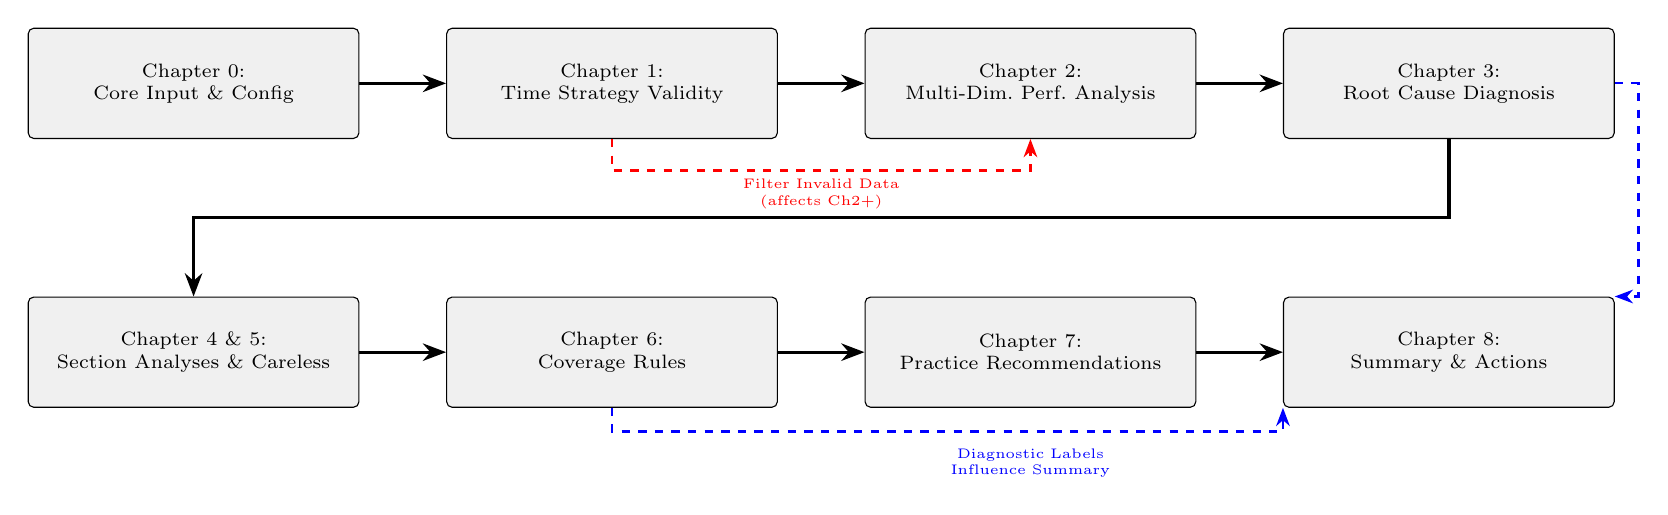
\begin{tikzpicture}[
  % --- styles ------------------------------------------------------------
  box/.style={
    rectangle, draw, rounded corners=2pt,
    minimum width=4.2cm, minimum height=1.4cm,
    font=\scriptsize, align=center, fill=gray!12
  },
  flow/.style={-Stealth, very thick},
  auxred/.style={-Stealth, dashed, red, thick},
  auxblue/.style={-Stealth, dashed, blue, thick},
  node distance = 2.0cm and 1.1cm % Vertical and horizontal node distance
]

% --------------------- 1st row ------------------------------------------
\node[box] (ch0) {Chapter 0:\\Core Input \& Config};
\node[box, right=of ch0] (ch1) {Chapter 1:\\Time Strategy Validity};
\node[box, right=of ch1] (ch2) {Chapter 2:\\Multi‑Dim.\ Perf.\ Analysis};
\node[box, right=of ch2] (ch3) {Chapter 3:\\Root Cause Diagnosis};

% --------------------- 2nd row ------------------------------------------
\node[box, below=of ch0] (ch4) {Chapter 4 \& 5:\\Section Analyses \& Careless}; % Standard space used
\node[box, right=of ch4] (ch6) {Chapter 6:\\Coverage Rules};
\node[box, right=of ch6] (ch7) {Chapter 7:\\Practice Recommendations};
\node[box, right=of ch7] (ch8) {Chapter 8:\\Summary \& Actions};

% --------------------- main flow arrows ---------------------------------
\draw[flow] (ch0) -- (ch1);
\draw[flow] (ch1) -- (ch2);
\draw[flow] (ch2) -- (ch3);

% ch3 -> ch4 (go down then left to avoid crossing the first row)
\coordinate (downR) at ($(ch3.south)+(0,-1)$); % Reduced vertical drop slightly
\coordinate (downL) at ($(ch4.north)+(0,0.4)$);
\draw[flow] (ch3.south) -- (downR) -- node[midway, below, font=\tiny] {} (downR -| ch4.north) -- (ch4.north); % Adjusted path

\draw[flow] (ch4) -- (ch6);
\draw[flow] (ch6) -- (ch7);
\draw[flow] (ch7) -- (ch8);

% --------------------- red auxiliary arrow ------------------------------
%  Vertical drop from ch1, then horizontal to ch2.south
\draw[auxred]
  ($(ch1.south)+(0,0)$) |- ($(ch1.south)+(0,-0.4)$) -| (ch2.south);

\node[font=\tiny, red, text width=2.7cm, align=center]
     at ($(ch1.south)!0.5!(ch2.south) + (0,-0.7)$) % Adjusted y-offset
     {Filter Invalid Data (affects Ch2+)};

% --------------------- blue diagnostic loop -----------------------------
% ch3 -> ch8
\draw[auxblue] (ch3.east) -- ++(0.3,0) |- (ch8.north east); % Simplified path

% ch6 -> ch8
\draw[auxblue] (ch6.south) -- ++(0,-0.3) -| (ch8.south west); % Simplified path

\node[font=\tiny, blue, text width=2.7cm, align=center]
     at ($(ch6.south)!0.5!(ch8.south) + (0,-0.7)$) % Adjusted y-offset
     {Diagnostic Labels\\Influence Summary};

\end{tikzpicture}} % End of \scalebox

\vspace{\baselineskip} % Vertical space added here

\caption{Overall Flow of the Unified Diagnostic Framework}
\label{fig:framework_flow}
\end{figure}
% ***** END OF FIGURE CODE *****

By applying this unified framework, students and instructors can gain a holistic understanding of performance, identify specific areas requiring intervention, and develop targeted strategies for improvement throughout the GMAT exam. The subsequent sections detail the methodology applied within each chapter of this framework.

\textit{Note on Document Purpose:} This document serves primarily as a technical report detailing the design, logic, and implementation rationale behind the unified GMAT diagnostic framework. It is intended as comprehensive documentation for users of the associated analysis tools (e.g., on GitHub) and as a methodological reference outlining the systematic approach developed. While initial parameters are informed by practical experience and preliminary testing, the core contribution presented here is the formalization of the diagnostic process itself.

Although experienced GMAT instructors often provide valuable information based on score reports, traditional analysis can suffer from subjectivity and inconsistency. Relying solely on intuition or anecdotal patterns introduces variability and hinders iterative refinement. Recognizing these limitations, the main motivation behind developing this unified diagnostic framework was to establish a more scientific, systematic, and objective approach. The goal is to enhance the efficiency, accuracy, and reliability of GMAT performance diagnosis by replacing purely experiential interpretation with a structured, parameterized, and verifiable methodology.

\section{Methodology: The Diagnostic Framework}

\subsection{Framework Development Methodology} % Replacing existing content

The development of this unified diagnostic framework originated from the practical need to structure insights gained through analyzing student GMAT performance, combining quantitative score report data with qualitative follow-up. Initial quantitative analysis relied on custom logic applied to performance metrics, while qualitative assessment, such as comparing student approaches to specific problems, aimed to uncover cognitive obstacles not evident in the raw data.

To establish a replicable process, consultations were transcribed and analyzed, utilizing AI assistance to consolidate the underlying analytical logic and structure. A key phase involved the explicit formalization of the diagnostic workflow, transforming subjective or ambiguous rules (e.g., "significant time pressure") into precise, parameterized definitions and functions. The outputs of this logic were designed as computable diagnostic tags, facilitating the generation of recommendations or guiding further qualitative inquiry.

Validation proceeded iteratively by comparing the framework's automated analysis against independent expert evaluations on real data. Discrepancies informed refinements to the logic, parameters, and functions, ensuring closer alignment with established diagnostic practices. The core framework was subsequently implemented as an automated tool using Python, a process involving learning logical control flow, modular design, and debugging techniques.

Throughout development, considerations for end-users—both students seeking intuitive interaction and instructors requiring detailed, traceable diagnostics—influenced design choices, leading to concepts like AI-assisted interfaces and standardized output tagging. This process highlighted that while AI can assist, the core analytical logic must be soundly defined by the expert. It also emphasized the need for maintainable code structure when dealing with AI-generated or complex components.

This narrative provides context for the detailed methodology presented in the subsequent chapters.

% The next subsection starts here:
\subsection{Chapter 0: Core Input Data and Configuration}

\textbf{Objective:} Define the foundational data structures, parameters, and pre-processing steps required for analysis.

\textbf{Required Input CSV Structure:}
For the analysis scripts to function correctly, the input CSV file (e.g., \texttt{testset-q.csv}) must contain specific columns with data in the expected format. While column names can sometimes be adapted during implementation, the following represents the ideal structure and data types:

\begin{itemize}
    \item \texttt{question\_position}: Sequence number of the question in the test (Integer, 1-indexed, serves as unique identifier).
    \item \texttt{question\_time}: Response time for the question in minutes (Numeric, Float).
    \item \texttt{is\_correct}: Indicator of correctness (Boolean: \texttt{True}/\texttt{False}).
    \item \texttt{content\_domain}: Classification as 'Math Related' or 'Non-Math Related' (String, DI only).
    \item \texttt{question\_type}: Category of the question (String). Specific values depend on the section:
        \begin{itemize}
            \item Q: 'Real' or 'Pure'.
            \item DI: 'DS', 'TPA', 'MSR', or 'GT'.
            \item V: 'CR' or 'RC'.
        \end{itemize}
    \item \texttt{msr\_group\_id}: MSR group identifier (Required only for MSR questions in DI section).
    \item \texttt{question\_difficulty}: Numeric difficulty value (Numeric). The source might differ (e.g., \texttt{DI\_b}, \texttt{V\_b}), but it's mapped internally.
    \item \texttt{question\_fundamental\_skill}: Core skill or domain tested (String, Required for Q and V, e.g., 'Rates/Ratio/Percent', 'Identify Stated Idea'). \textbf{Note: Fundamental Skills are NOT tracked for DI.}
\end{itemize}

\textbf{Overall Metrics (Derived or Input):}
While not always direct columns, the analysis requires:
\begin{itemize}
    \item \texttt{total\_test\_time}: Total minutes spent (45 minutes standard).
    \item \texttt{max\_allowed\_time}: Standard 45 minutes per section.
    \item \texttt{total\_number\_of\_questions}: 20 questions for DI, varies for Q/V.
\end{itemize}

\textbf{Section-Specific Inputs \& Pre-processing:}
\begin{itemize}
    \item \textbf{Quant (Q):}
    \begin{itemize}
        \item Inputs: \texttt{question\_type} categorized as 'Real' (word problems) or 'Pure' (computation/concept); \texttt{question\_fundamental\_skill} representing core mathematical areas, e.g.:
            \begin{itemize}
                \item \texttt{Rates/Ratio/Percent}
                \item \texttt{Value/Order/Factor}
                \item \texttt{Equal/Unequal/ALG}
                \item \texttt{Counting/Sets/Series/Prob/Stats}
            \end{itemize}
        \item Pre-processing: Calculate \texttt{average\_time\_per\_type}, \texttt{max\_correct\_difficulty\_per\_skill}. Numerical conversions and handling of missing values are performed.
    \end{itemize}
    \item \textbf{Data Insights (DI):}
    \begin{itemize}
        \item \textbf{Basic Settings:} \texttt{Max Allowed Time}: 45 minutes; \texttt{Total Number of Questions}: 20.
        \item \textbf{Question Type Abbreviations:} \texttt{DS}: Data Sufficiency; \texttt{TPA}: Two-Part Analysis; \texttt{MSR}: Multi-Source Reasoning; \texttt{GT}: Graph \& Table.
        \item Inputs: \texttt{question\_type} ('DS', 'TPA', 'MSR', 'GT'); \texttt{content\_domain} ('Math Related'/'Non-Math Related'); \texttt{msr\_group\_id} (required if \texttt{question\_type} is 'MSR'). \textbf{Note: Fundamental Skills are typically NOT tracked for DI.}
        \item \textbf{DI Derived Data Pre-processing:}
        \begin{itemize}
            \item \textbf{MSR Reading Time (\texttt{msr\_reading\_time}):} For each MSR group, calculate reading time as: first question's \texttt{question\_time} minus average \texttt{question\_time} of all other questions in the group. This calculation is only valid when the group contains at least two questions, and the result is attached to the first question of the group. (This data will be used in Chapter 1 for MSR single question overtime judgment.)
            \item \textbf{MSR Group Data Pre-calculation:}
                \begin{itemize}
                    \item \texttt{group\_total\_time}: Sum of \texttt{question\_time} for all questions in each MSR group.
                    \item \texttt{num\_q\_in\_group}: Number of questions in each MSR group.
                \end{itemize}
            \item \textbf{GT Time Allocation:} No special distinction between graph viewing and answering time.
            \item \textbf{Average Time per Type (\texttt{average\_time\_per\_type}):} Calculate average \texttt{question\_time} for each \texttt{question\_type} ('DS', 'TPA', 'MSR', 'GT') based on filtered valid data. (This data will be used in Chapter 3 for defining \texttt{is\_relatively\_fast} and Chapter 4 for carelessness rate calculation.)
            \item \textbf{First Third Average Time per Type (\texttt{first\_third\_average\_time\_per\_type}):} For each \texttt{question\_type} ('DS', 'TPA', 'MSR', 'GT'), calculate average \texttt{question\_time} for all questions where \texttt{question\_position} $\leq$ (\texttt{Total Number of Questions} / 3). (This data will be used in Chapter 1 for invalid data judgment.)
            \item \textbf{Max Mastered Difficulty per Combination (\texttt{max\_correct\_difficulty\_per\_combination}):} 
            For each \texttt{question\_type} and \texttt{content\_domain} combination, \\
            record the highest \texttt{question\_difficulty} value among all questions where \texttt{is\_correct} == \texttt{True}.
        \end{itemize}
    \end{itemize}
    \item \textbf{Verbal (V):}
    \begin{itemize}
        \item Inputs: \texttt{question\_type} ('CR'/'RC'); \texttt{question\_fundamental\_skill}, e.g.:
            \begin{itemize}
                \item \texttt{Plan/Construct}
                \item \texttt{Identify Stated Idea}
                \item \texttt{Identify Inferred Idea}
                \item \texttt{Analysis/Critique}
            \end{itemize}
        \item Pre-processing: Identify \texttt{RC} passage groups (consecutive RC questions, usually 3-4). Calculate the following:
            \begin{itemize}
                \item \texttt{rc\_group\_id}
                \item \texttt{questions\_in\_group}
                \item \texttt{group\_total\_time}
                \item \texttt{average\_time\_per\_type}
                \item \texttt{first\_third\_average\_time\_per\_type}
            \end{itemize}
            Estimate \texttt{rc\_reading\_time} using a similar logic to MSR:
            \texttt{reading\_time = time\_q1 - average\_time\_of\_other\_qs\_in\_group}.
    \end{itemize}
\end{itemize}

\textbf{Implementation Context:} Data ingestion typically involves reading CSV files using libraries like \texttt{pandas}. Pre-processing includes data type conversion (e.g., \texttt{pd.to\_numeric}), handling missing data (\texttt{dropna}), mapping raw inputs (e.g., full question type names to abbreviations like 'DS'), renaming columns for consistency, and computing the derived metrics mentioned above. Configuration parameters (thresholds, factors) are defined constants within the implementation.

\textbf{Rationale:} Establishes a consistent, clean, and enriched data foundation crucial for reliable and comparable diagnostics across sections, with particular attention to DI-specific requirements such as MSR group processing and content domain classification.

\subsection{Chapter 1: Overall Time Strategy and Data Validity Assessment}

\textbf{Objective:} Evaluate overall pacing, assess time pressure, establish section-appropriate overtime criteria, and identify potentially invalid data points resulting from rushed end-section performance.

\textbf{Operational Logic:}
\begin{enumerate}
    \item \textbf{Calculate Time Difference (\texttt{time\_diff}):} Computed as \texttt{max\_allowed\_time} - \texttt{total\_test\_time}.
    \item \textbf{Determine Time Pressure Status (\texttt{time\_pressure}):} This Boolean flag indicates potential time pressure during the test section. 
        \begin{itemize}
            \item Default: \texttt{time\_pressure} = \texttt{False}.
            \item Check end-section conditions: Find questions in the last 1/3 of the test (\texttt{last\_third\_questions}) where \texttt{question\_time} $<$ 1.0 minute (\texttt{fast\_end\_questions}).
            \item Judgment Logic: If \texttt{time\_diff} $\leq$ 3 minutes \textbf{AND} \texttt{fast\_end\_questions} is not empty, then set \texttt{time\_pressure} = \texttt{True}.
            \item \textbf{User Override:} If user explicitly indicates low pressure, force \texttt{time\_pressure} = \texttt{False}.
        \end{itemize}
    \item \textbf{Establish Overtime Thresholds/Rules (Based on \texttt{time\_pressure}):} These criteria are dynamically set based on the \texttt{time\_pressure} status and vary by section and question type.
    \begin{itemize}
        \item \textbf{Q:} A single \texttt{overtime\_threshold} (e.g., 2.5 min if \texttt{time\_pressure}, 3.0 min otherwise).
        \item \textbf{DI:} Type-specific thresholds and MSR group rules:
        \begin{itemize}
            \item \textbf{TPA Overtime Threshold (\texttt{overtime\_threshold\_tpa}):} 3.0 min if \texttt{time\_pressure} == \texttt{True}; 3.5 min if \texttt{time\_pressure} == \texttt{False}.
            \item \textbf{GT Overtime Threshold (\texttt{overtime\_threshold\_gt}):} 3.0 min if \texttt{time\_pressure} == \texttt{True}; 3.5 min if \texttt{time\_pressure} == \texttt{False}.
            \item \textbf{DS Overtime Threshold (\texttt{overtime\_threshold\_ds}):} 2.0 min if \texttt{time\_pressure} == \texttt{True}; 2.5 min if \texttt{time\_pressure} == \texttt{False}.
            \item \textbf{MSR Group Target Time Rules (\texttt{msr\_group\_target\_time}):} 6.0 min if \texttt{time\_pressure} == \texttt{True}; 7.0 min if \texttt{time\_pressure} == \texttt{False}.
            \item \textbf{MSR Single Question Analysis Thresholds:}
                \begin{itemize}
                    \item \texttt{msr\_reading\_threshold}: 1.5 minutes (for judging if reading time is excessive).
                    \item \texttt{msr\_single\_q\_threshold}: 1.5 minutes (for judging if single question answering time is excessive).
                \end{itemize}
        \end{itemize}
        \item \textbf{V:} Separate thresholds/rules for \texttt{CR} (\texttt{overtime\_threshold\_cr}: 2.0 min if \texttt{time\_pressure}, 2.5 otherwise) and \texttt{RC} (e.g., \texttt{rc\_group\_target\_time} for 3Q group: 6.0 min if \texttt{time\_pressure}, 7.0 otherwise; for 4Q group: 8.0 min if \texttt{time\_pressure}, 9.0 otherwise; \texttt{rc\_individual\_q\_threshold}=2.0 min). V also includes a preliminary check for \texttt{reading\_comprehension\_barrier\_inquiry} based on estimated \texttt{rc\_reading\_time} exceeding thresholds (e.g., >2.0 min for 3Q group, >2.5 min for 4Q group).
    \end{itemize}
    \item \textbf{Identify Invalid Data (\texttt{is\_invalid}):} This flag identifies questions likely answered without genuine effort due to time constraints.
        \begin{itemize}
            \item \textbf{Trigger Condition:} Only executed if \texttt{time\_pressure} == \texttt{True}. If \texttt{time\_pressure} == \texttt{False}, no questions are marked as \texttt{is\_invalid}.
            \item \textbf{Scope:} Only checks questions in the final third (\texttt{last\_third\_questions}).
            \item \textbf{Definition of "Abnormally Fast Response" (\texttt{abnormally\_fast\_response}) Standards (meeting any one triggers):}
                \begin{itemize}
                    \item \textit{Standard 1 (Suspected abandonment):} \texttt{question\_time} $<$ 0.5 minutes.
                    \item \textit{Standard 2 (Absolute rush):} \texttt{question\_time} $<$ 1.0 minute.
                    \item \textit{Standard 3 (Relative single question rush - DS):} \texttt{question\_time} $<$ (\texttt{first\_third\_average\_time\_per\_type}['DS'] * 0.5).
                    \item \textit{Standard 4 (Relative single question rush - TPA):} \texttt{question\_time} $<$ (\texttt{first\_third\_average\_time\_per\_type}['TPA'] * 0.5).
                    \item \textit{Standard 5 (Relative single question rush - GT):} \texttt{question\_time} $<$ (\texttt{first\_third\_average\_time\_per\_type}['GT'] * 0.5).
                    \item \textit{Standard 6 (Relative group rush - MSR):} The MSR group containing the question has \texttt{group\_total\_time} $<$ (\texttt{first\_third\_average\_time\_per\_type}['MSR'] * \texttt{num\_q\_in\_group} * 0.5).
                \end{itemize}
            \item \textbf{Marking Logic:} Within the \texttt{last\_third\_questions} scope, if a question (or its MSR group for Standard 6) meets \textbf{at least one} \texttt{abnormally\_fast\_response} standard, \textbf{and \texttt{time\_pressure} == \texttt{True}}, then mark that question as \texttt{is\_invalid} = \texttt{True}.
        \end{itemize}
    \item \textbf{Global Rule - Data Filtering and Overtime Flagging:}
    \begin{itemize}
        \item \textbf{Mark Overtime (\texttt{overtime}):} Based on the thresholds/rules defined in this chapter, mark \texttt{overtime} = \texttt{True} for all questions \textbf{not marked as \texttt{is\_invalid}}.
        \item \textbf{DI-Specific MSR Overtime Marking (Four-tier Standards):}
            \begin{itemize}
                \item \textbf{a. Group Overtime Marking (\texttt{msr\_group\_over}):} Calculate total time (\texttt{msr\_group\_total\_time}) for each MSR group. If \texttt{msr\_group\_total\_time} $>$ \texttt{msr\_group\_target\_time}, mark \textbf{all} questions in that MSR group as \texttt{msr\_group\_over} = \texttt{True}.
                \item \textbf{b. Reading Time Overtime Marking (\texttt{msr\_reading\_over}):} For MSR questions that are \textbf{not marked by \texttt{msr\_group\_over}} and are \textbf{first questions in their group}: if \texttt{msr\_reading\_time} $>$ \texttt{msr\_reading\_threshold} (1.5 minutes), mark \texttt{msr\_reading\_over} = \texttt{True}.
                \item \textbf{c. Adjusted First Question Overtime Marking (\texttt{msr\_adj\_first\_over}):} For MSR questions that are \textbf{not marked by the above two conditions} and are \textbf{first questions in their group}: calculate \texttt{adjusted\_time} = \texttt{question\_time} - \texttt{msr\_reading\_time}. If \texttt{adjusted\_time} $>$ \texttt{msr\_single\_q\_threshold} (1.5 minutes), mark \texttt{msr\_adj\_first\_over} = \texttt{True}.
                \item \textbf{d. Non-First Question Overtime Marking (\texttt{msr\_non\_first\_over}):} For MSR questions that are \textbf{not marked by \texttt{msr\_group\_over}} and are \textbf{not first questions in their group}: if \texttt{question\_time} $>$ \texttt{msr\_single\_q\_threshold} (1.5 minutes), mark \texttt{msr\_non\_first\_over} = \texttt{True}.
                \item \textbf{e. Final \texttt{overtime} Marking:} An MSR question is finally marked as \texttt{overtime} = \texttt{True} if and only if it meets any of these conditions: \texttt{msr\_group\_over} OR \texttt{msr\_reading\_over} OR \texttt{msr\_adj\_first\_over} OR \texttt{msr\_non\_first\_over}.
            \end{itemize}
        \item \textbf{Create Filtered Dataset:} Remove all questions marked as \texttt{is\_invalid} = \texttt{True} from the original question data.
        \item \textbf{Subsequent Analysis Scope:} All analysis in Chapters 2-6 is based exclusively on this filtered dataset.
    \end{itemize}
\end{enumerate}

% ***** FIGURE: Chapter 1 Logic *****
    \begin{figure}[htbp]
    \centering
    % --- Use \scalebox to scale the chart ---
    \scalebox{0.65}{ % Adjusted scale factor slightly, try values like 0.6, 0.7 if needed
    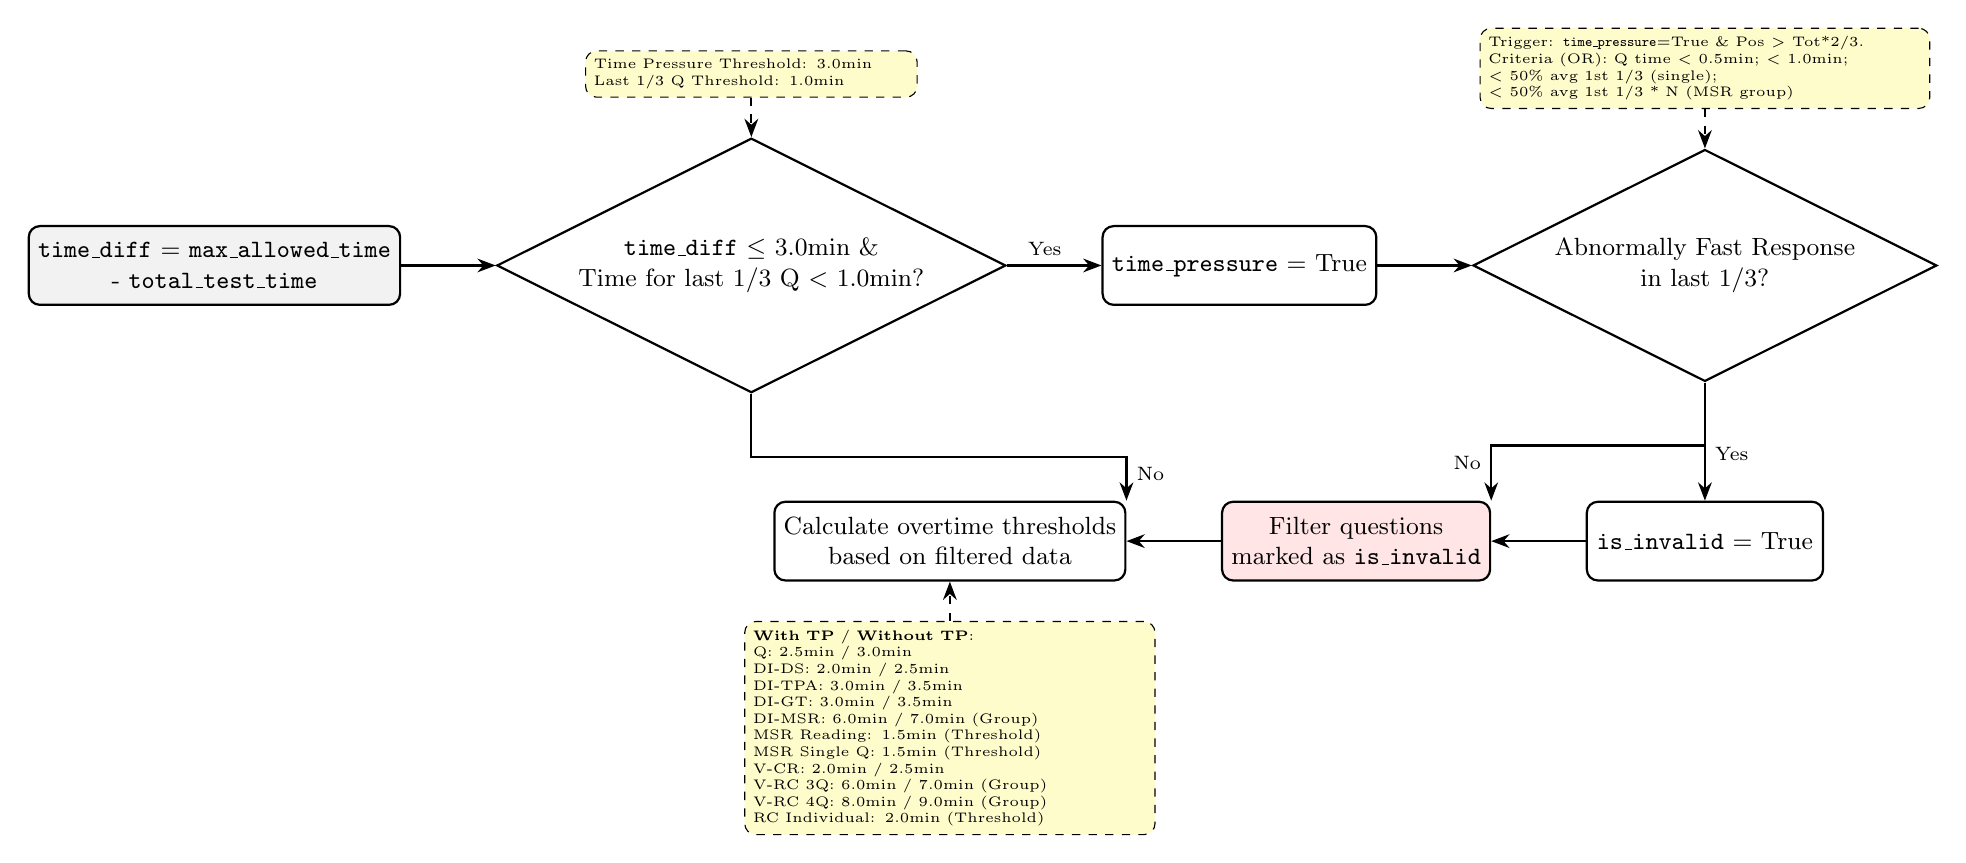
\begin{tikzpicture}[
        box/.style={rectangle, draw, rounded corners, minimum width=3cm, minimum height=1cm, text centered, font=\small, align=center, thick},
        decision/.style={diamond, draw, aspect=2, minimum width=4cm, minimum height=1.5cm, text centered, font=\small, align=center, thick},
        arrow/.style={-Stealth, thick}, % Changed to -Stealth
        param/.style={rectangle, draw, dashed, rounded corners, fill=yellow!20, font=\tiny, align=left, inner sep=3pt, text width=4.5cm}, % Increased inner sep, added text width
        % Adjust node distance for layout
        node distance=1.8cm and 1.2cm % Adjusted vertical and horizontal distance
    ]
    % Nodes - Row 1 (Left to Right)
    \node[box, fill=gray!10] (time_diff) {\texttt{time\_diff} = \texttt{max\_allowed\_time} \\ - \texttt{total\_test\_time}};

    % CORRECTED: Added $ signs around <= and <
    \node[decision, right=of time_diff] (pressure_cond) {\texttt{time\_diff} $\leq$ 3.0min \&\\ Time for last 1/3 Q $<$ 1.0min?}; % Ampersand & line break

    \node[box, right=of pressure_cond] (pressure_result) {\texttt{time\_pressure} = True};

    \node[decision, right=of pressure_result] (invalid_check) {Abnormally Fast Response\\ in last 1/3?}; % MODIFIED NODE TEXT

    % Nodes - Row 2 (Connect right-to-left below, slight shift)
    \node[box, below = 1.5cm of invalid_check] (invalid_result) {\texttt{is\_invalid} = True}; % Increased vertical distance slightly

    \node[box, fill=red!10, left=of invalid_result] (filter) {Filter questions\\ marked as \texttt{is\_invalid}};

    \node[box, left=of filter] (overtime) {Calculate overtime thresholds\\ based on filtered data};

    % Parameter Nodes (Positioned below main nodes they relate to)
    % CORRECTED: Added $ signs around <
    \node[param, above = 0.5cm of pressure_cond, text width=4cm] (pressure_param) {Time Pressure Threshold: 3.0min\\ Last 1/3 Q Threshold: 1.0min};

    % CORRECTED: Added $ signs around > and <
    \node[param, above = 0.5cm of invalid_check, text width=5.5cm] (invalid_param) {Trigger: \texttt{time\_pressure}=True \& Pos $>$ Tot*2/3.\\ Criteria (OR): Q time $<$ 0.5min; $<$ 1.0min;\\ $<$ 50\% avg 1st 1/3 (single);\\ $<$ 50\% avg 1st 1/3 * N (MSR group)}; % MODIFIED PARAM TEXT, explicit text width

    \node[param, below = 0.5cm of overtime, text width=5cm] (overtime_params) { % Explicit text width
        \textbf{With TP} / \textbf{Without TP}:\\ % TP = Time Pressure
        Q: 2.5min / 3.0min\\
        DI-DS: 2.0min / 2.5min\\
        DI-TPA: 3.0min / 3.5min\\
        DI-GT: 3.0min / 3.5min\\ % CONFIRMED THRESHOLD
        DI-MSR: 6.0min / 7.0min (Group)\\
        MSR Reading: 1.5min (Threshold)\\
        MSR Single Q: 1.5min (Threshold)\\
        V-CR: 2.0min / 2.5min\\
        V-RC 3Q: 6.0min / 7.0min (Group)\\
        V-RC 4Q: 8.0min / 9.0min (Group)\\
        RC Individual: 2.0min (Threshold)
    };

    % Connections - Flow
    \draw[arrow] (time_diff) -- (pressure_cond);
    \draw[arrow] (pressure_cond) -- node[above, font=\scriptsize, pos=0.4] {Yes} (pressure_result);
    \draw[arrow] (pressure_result) -- (invalid_check);
    % Decision branches
    \draw[arrow] (pressure_cond.south) |- ++(0,-0.8) -| node[midway, below right, font=\scriptsize] {No} (overtime.north east); % "No" path for pressure

    \draw[arrow] (invalid_check) -- node[right, font=\scriptsize, pos=0.6] {Yes} (invalid_result); % Down arrow for "Yes"
    \draw[arrow] (invalid_result) -- (filter); % Left arrow
    \draw[arrow] (filter) -- (overtime); % Left arrow

    % "No" path for invalid check
    \draw[arrow] (invalid_check.south) |- ++(0,-0.8) -| node[midway, below left, font=\scriptsize] {No} (filter.north east); % Directly to filter if not invalid

    % Parameter Connections (dashed)
    \draw[arrow, dashed] (pressure_param) -- (pressure_cond);
    \draw[arrow, dashed] (invalid_param) -- (invalid_check);
    \draw[arrow, dashed] (overtime_params) -- (overtime);

    \end{tikzpicture}
    } % <-- End of \scalebox
    % --- End \scalebox ---

    \vspace{\baselineskip} % Space between figure and caption
    \caption{Flowchart for Chapter 1 Logic: Time Pressure, Data Validity, and Overtime Thresholds}
    \label{fig:chapter1_logic}
    \end{figure}
    % ***** END OF FIGURE CODE *****

\textbf{Implementation Context:} Boolean flags (\texttt{time\_pressure}, \texttt{is\_invalid}, \texttt{overtime}) are added as columns to the \texttt{pandas} DataFrame. Thresholds are assigned to variables based on conditional logic applied to the \texttt{time\_pressure} status. Filtering is achieved via DataFrame slicing (e.g., \texttt{df\_filtered = df[$\sim$df['is\_invalid']]}). For DI section, special handling is required for MSR questions with the four-tier overtime marking system.

\textbf{Rationale:} Ensures analyses are based on reliable data reflecting genuine effort and capability, while setting context-aware standards for time efficiency. Explicitly filtering invalid data before overtime flagging prevents misinterpreting rushed guesses as slow performance. The sophisticated MSR overtime detection system accounts for the unique structure and timing requirements of Multi-Source Reasoning questions.

\subsection{Chapter 2: Multi-Dimensional Performance Analysis}

\textbf{Objective:} Analyze performance accuracy and efficiency across key dimensions relevant to each section, using the \textbf{filtered dataset}.

\textbf{Operational Logic:}
\begin{itemize}
    \item \textbf{Difficulty Level Standardization:} Raw numeric \texttt{question\_difficulty} values are mapped to standardized categorical bands (e.g., "Low / 505+", "Medium / 605+", "High / 705+") using a consistent mapping function across sections. This facilitates comparison and interpretation.
    \item \textbf{Performance Metric Calculation:} For each relevant dimension or combination, calculate key metrics using the filtered data: total count, number of errors (\texttt{is\_correct}==\texttt{False}), number of overtime instances (\texttt{overtime}==\texttt{True}), error rate, and overtime rate. Division by zero is handled gracefully (e.g., returning 0.0 or NaN).
\end{itemize}

% \newpage % Consider removing forced page breaks unless necessary for final layout
\textbf{Section-Specific Analysis Dimensions \& Metrics:}
\begin{itemize}
    \item \textbf{Quant (Q):}
    \begin{itemize}
        \item The primary dimensions analyzed for Quant section are: \texttt{question\_type} ('Real'/'Pure'), \texttt{question\_fundamental\_skill}, and \texttt{difficulty\_label}.
        \item Analysis: Compares error rates and overtime rates between 'Real' and 'Pure'. Identifies significant differences based on absolute count difference ($\geq$ 2) in errors or overtime instances, setting flags (\texttt{poor\_real}, \texttt{slow\_pure}, etc.). % CORRECTED: Added $ sign
    \end{itemize}
    \item \textbf{Data Insights (DI):}
    \begin{itemize}
        \item Dimensions: \texttt{content\_domain} ('Math Related'/'Non-Math Related'), \texttt{question\_type} ('DS', 'TPA', 'MSR', 'GT'), \texttt{difficulty\_label}.
        \item Analysis: Calculates error and overtime rates per dimension/combination. Identifies significant differences between \texttt{content\_domain}s based on absolute count difference ($\geq$ 2), setting flags (\texttt{poor\_math\_related}, \texttt{slow\_non\_math\_related}, etc.). % CORRECTED: Added $ sign
    \end{itemize}
    \item \textbf{Verbal (V):}
    \begin{itemize}
        \item Dimensions: \texttt{question\_fundamental\_skill}, \texttt{difficulty\_label}, \texttt{question\_type} ('CR'/'RC').
        \item Analysis: Calculates error rates per dimension/combination. Identifies difficulty ranges and skills with the highest error concentration.
    \end{itemize}
\end{itemize}

\textbf{Implementation Context:} \texttt{pandas} \texttt{groupby()} operations combined with \texttt{agg()} or \texttt{size().unstack()} are used extensively to compute metrics across dimensions. Error and overtime rates are calculated element-wise, often requiring intermediate steps to handle potential zero denominators (e.g., replacing 0 with \texttt{np.nan} before division). Significance flags are set using conditional logic based on the calculated metric differences.

\textbf{Rationale:} Pinpoint specific areas (types, skills, domains, difficulties) where accuracy or efficiency challenges exist within the valid performance data, providing focus for root cause diagnosis and practice planning.

\subsection{Chapter 3: Root Cause Diagnosis and Analysis}

\textbf{Objective:} Investigate the underlying reasons (\"why") for errors and inefficiencies identified in previous chapters, utilizing the \textbf{filtered dataset}.

\textbf{Core Concepts \& Operational Framework:}
\begin{enumerate}
    \item \textbf{Time Performance Classification:} Categorizes each valid question\'s time relative to the average for its type. Required metrics (\texttt{average\_time\_per\_type}) are pre-calculated from the filtered data.
    \begin{itemize}
        \item \texttt{is\_relatively\_fast}: \texttt{question\_time} $<$ (\texttt{average\_time\_per\_type} * 0.75). The 0.75 factor is a configurable parameter. % CORRECTED: Added $ sign
        \item \texttt{is\_slow}: Determined by the \texttt{overtime} flag (or its variants) applied in Chapter 1 based on the filtered data.
        \item \texttt{is\_normal\_time}: Default state if neither \texttt{is\_relatively\_fast} nor \texttt{is\_slow}.
    \end{itemize}
    \item \textbf{Special Focus Error (\texttt{special\_focus\_error}, SFE):} This critical flag identifies instability in foundational knowledge.
    \begin{itemize}
        \item Definition: An error is classified as SFE under the following condition:
        \texttt{is\_correct} == False AND \texttt{question\_difficulty} $<$ \texttt{max\_mastered\_difficulty}. % CORRECTED: Added $ sign
        \item \texttt{max\_mastered\_difficulty} is calculated per \texttt{question\_fundamental\_skill} (for Q/V) or per \texttt{question\_type}/\texttt{content\_domain} combination (for DI section) by finding the maximum \texttt{question\_difficulty} among correctly answered questions within that category in the filtered data.
        \item Handling: SFE-flagged questions receive priority in subsequent reporting and recommendation generation.
    \end{itemize}
    \item \textbf{Diagnostic Label Assignment:} Based on the time performance classification and SFE status, each question is assigned diagnostic labels. These labels encapsulate the primary findings regarding potential root causes (e.g., \"Slow \& Wrong\", \"Fast \& Wrong\", \"SFE\"). These labels, rather than complex scenarios, serve as the core input for generating targeted recommendations in Chapter 7 and the narrative summary in Chapter 8. The detailed follow-up actions (student recall, evidence review, qualitative analysis) are presented as guidance in Chapter 8.
\end{enumerate}

% ***** FIGURE: Chapter 3 Logic (Modified with Diagonal Lines) *****
\begin{figure}[htbp]
\centering
% --- Scale box to manage width ---
\scalebox{0.65}{ % Adjusted scale factor, try 0.6 or 0.7 if needed
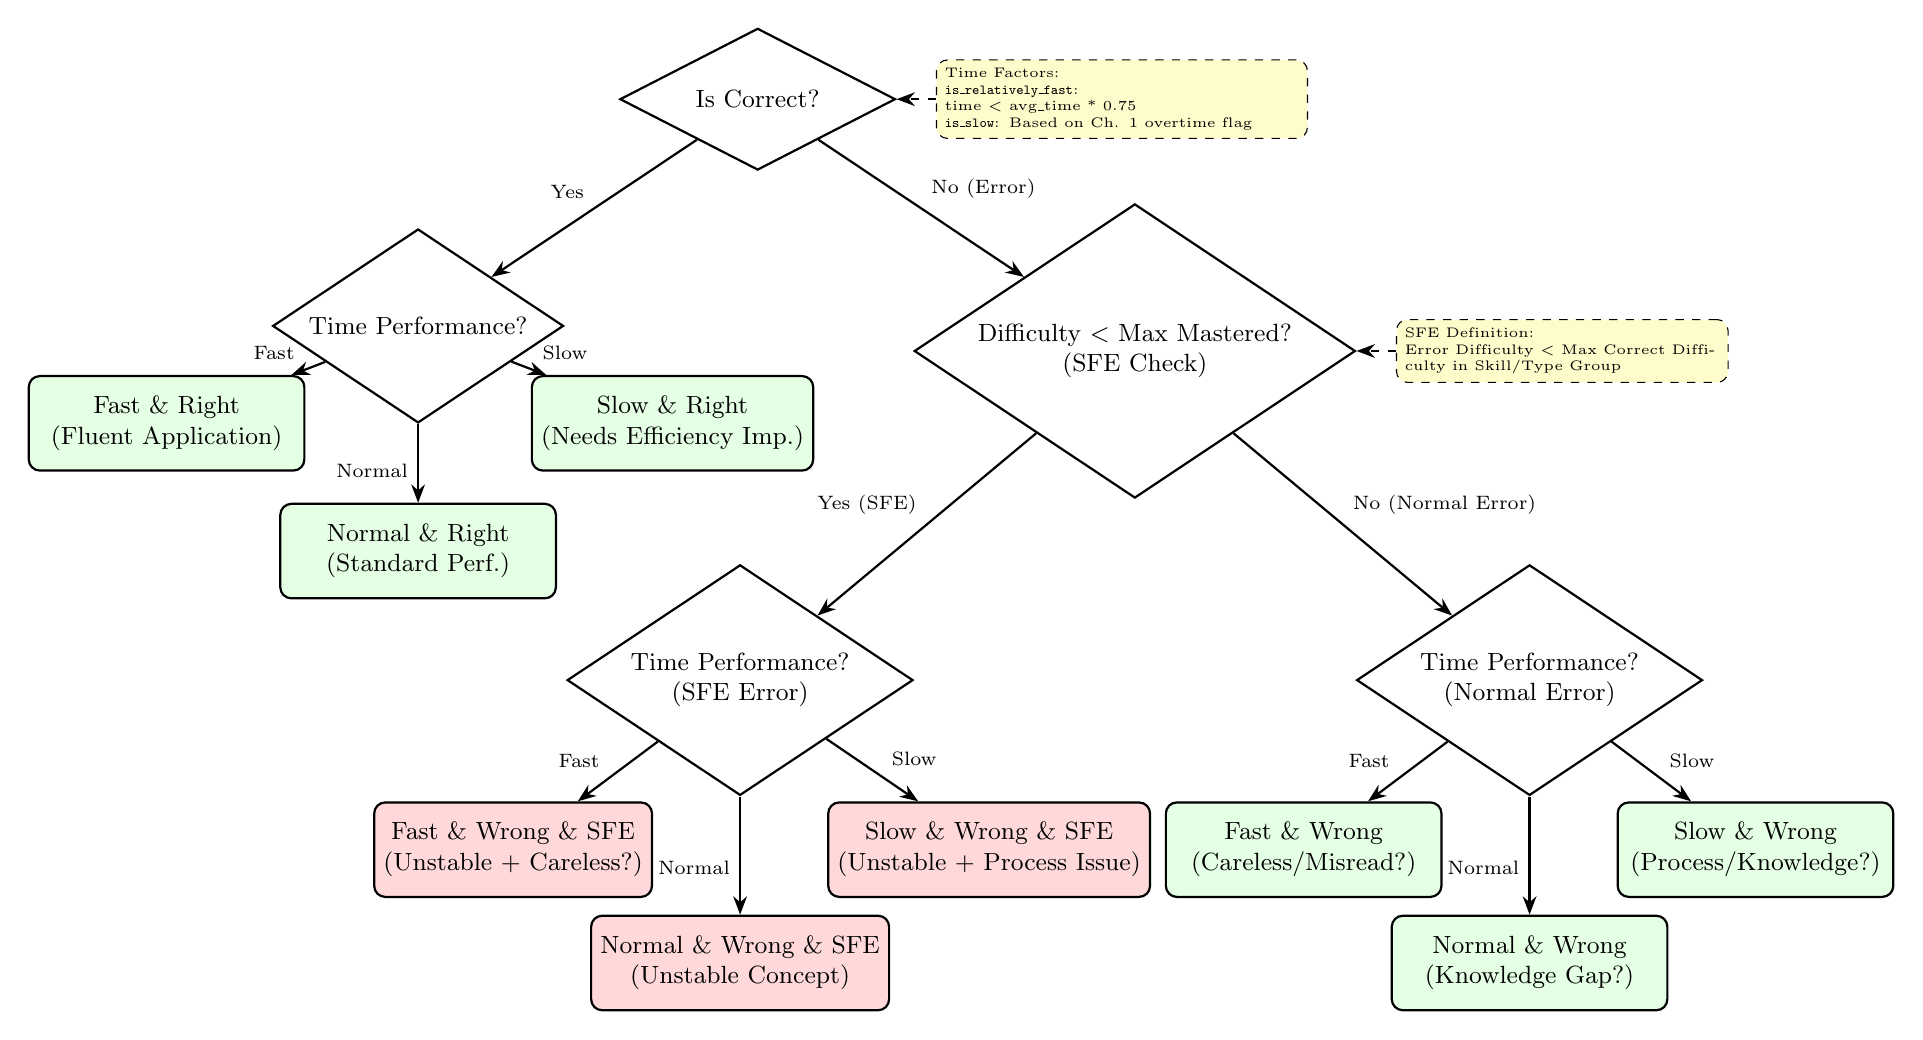
\begin{tikzpicture}[
    % General node distance (vertical and horizontal)
    node distance=1.8cm and 2.5cm, % Adjusted vertical and horizontal base distance
    % Styles
    decision/.style={diamond, draw, aspect=1.5, minimum width=3.5cm, minimum height=1.8cm, text centered, font=\small, align=center, thick},
    leaf/.style={rectangle, draw, rounded corners, fill=green!10, minimum width=3.5cm, minimum height=1.2cm, text centered, font=\small, align=center, thick},
    arrow/.style={-Stealth, thick}, % Changed to -Stealth
    param/.style={rectangle, draw, dashed, rounded corners, fill=yellow!20, font=\tiny, align=left, inner sep=3pt, text width=4cm} % Added text width
]
% --- Root Node and Parameters ---
\node[decision] (is_correct) {Is Correct?};

% CORRECTED: Added $ sign around <
\node[param, right = 0.5cm of is_correct, text width=4.5cm] (time_params) {Time Factors:\\\texttt{is\_relatively\_fast}: \\time $<$ avg\_time * 0.75\\\texttt{is\_slow}: Based on Ch. 1 overtime flag}; % Added text width
\draw[arrow, dashed] (time_params) -- (is_correct); % This was already a direct line

% --- Correct Branch ---
\node[decision, below left = of is_correct] (correct_time) {Time Performance?}; % Relative positioning
% MODIFIED LINE: Changed |- to -- and adjusted label position
\draw[arrow] (is_correct) -- node[above left, pos=0.5, font=\scriptsize] {Yes} (correct_time);

\node[leaf, below left = 0cm and 0.5cm of correct_time] (fast_right) {Fast \& Right\\(Fluent Application)}; % Adjusted position
\node[leaf, below = 1cm of correct_time] (normal_right) {Normal \& Right\\(Standard Perf.)};
\node[leaf, below right = 0cm and 0.5cm of correct_time] (slow_right) {Slow \& Right\\(Needs Efficiency Imp.)}; % Adjusted position

\draw[arrow] (correct_time) -- node[above left, font=\scriptsize, pos=0.6] {Fast} (fast_right);
\draw[arrow] (correct_time) -- node[left, font=\scriptsize, pos=0.6] {Normal} (normal_right); % Changed label position
\draw[arrow] (correct_time) -- node[above right, font=\scriptsize, pos=0.6] {Slow} (slow_right);

% --- Incorrect Branch ---
% CORRECTED: Added $ sign around <
\node[decision, below right = of is_correct] (wrong_first) {Difficulty $<$ Max Mastered? \\ (SFE Check)}; % Relative positioning, simpler text
% MODIFIED LINE: Changed |- to -- and adjusted label position
\draw[arrow] (is_correct) -- node[above right, pos=0.5, font=\scriptsize] {No (Error)} (wrong_first);

% CORRECTED: Added $ sign around <
\node[param, right = 0.5cm of wrong_first, text width=4cm] (sfe_param) {SFE Definition:\\ Error Difficulty $<$ Max Correct Difficulty in Skill/Type Group}; % Added text width
\draw[arrow, dashed] (sfe_param) -- (wrong_first); % This was already a direct line

% --- Sub-branches for Incorrect questions ---
\node[decision, below left = 2.5cm and 2.5cm of wrong_first] (sfe_time) {Time Performance? \\ (SFE Error)}; % Added context
\node[decision, below right = 2.5cm and 2.5cm of wrong_first] (normal_wrong_time) {Time Performance? \\ (Normal Error)}; % Added context

% MODIFIED LINE: Changed |- to -- and adjusted label position
\draw[arrow] (wrong_first) -- node[above left, pos=0.5, font=\scriptsize] {Yes (SFE)} (sfe_time);
% MODIFIED LINE: Changed |- to -- and adjusted label position
\draw[arrow] (wrong_first) -- node[above right, pos=0.5, font=\scriptsize] {No (Normal Error)} (normal_wrong_time);

% --- SFE Sub-branch Leaves (Adjust positioning relative to sfe_time) ---
\node[leaf, below left = 0.8cm and 0.0cm of sfe_time, fill=red!15] (fast_wrong_sfe) {Fast \& Wrong \& SFE\\(Unstable + Careless?)}; % Adjusted pos
\node[leaf, below = 1.5cm of sfe_time, fill=red!15] (normal_wrong_sfe) {Normal \& Wrong \& SFE\\(Unstable Concept)};
\node[leaf, below right = 0.8cm and 0.0cm of sfe_time, fill=red!15] (slow_wrong_sfe) {Slow \& Wrong \& SFE\\(Unstable + Process Issue)}; % Adjusted pos

\draw[arrow] (sfe_time) -- node[above left, font=\scriptsize, pos=0.6] {Fast} (fast_wrong_sfe);
\draw[arrow] (sfe_time) -- node[left, font=\scriptsize, pos=0.6] {Normal} (normal_wrong_sfe); % Changed label position
\draw[arrow] (sfe_time) -- node[above right, font=\scriptsize, pos=0.6] {Slow} (slow_wrong_sfe);

% --- Normal Wrong Sub-branch Leaves (Adjust positioning relative to normal_wrong_time) ---
\node[leaf, below left = 0.8cm and 0.0cm of normal_wrong_time] (fast_wrong) {Fast \& Wrong\\(Careless/Misread?)}; % Adjusted pos
\node[leaf, below = 1.5cm of normal_wrong_time] (normal_wrong) {Normal \& Wrong\\(Knowledge Gap?)};
\node[leaf, below right = 0.8cm and 0.0cm of normal_wrong_time] (slow_wrong) {Slow \& Wrong\\(Process/Knowledge?)}; % Adjusted pos

\draw[arrow] (normal_wrong_time) -- node[above left, font=\scriptsize, pos=0.6] {Fast} (fast_wrong);
\draw[arrow] (normal_wrong_time) -- node[left, font=\scriptsize, pos=0.6] {Normal} (normal_wrong); % Changed label position
\draw[arrow] (normal_wrong_time) -- node[above right, font=\scriptsize, pos=0.6] {Slow} (slow_wrong);

\end{tikzpicture}
} % <-- End of \scalebox
\vspace{\baselineskip} % Space between figure and caption
\caption{Flowchart for Chapter 3 Logic: Root Cause Diagnosis Labels (Diagonal Lines)} % Updated caption slightly
\label{fig:chapter3_logic_diagonal} % Changed label to avoid conflict if used alongside original
\end{figure}
% ***** END OF FIGURE CODE *****

\textbf{Implementation Context:} The logic is implemented within the main analysis loop iterating through the filtered DataFrame. Time classification and SFE flags (serving as primary diagnostic labels) are computed for each question. These labels are stored, often alongside brief descriptive notes derived from the combination (e.g., potential cause hypotheses like "calculation barrier" for DI Math Slow \& Wrong), for use in generating detailed diagnostic text and recommendations in Chapters 7 and 8.

\textbf{Rationale:} Moves beyond identifying \textit{what} is wrong to systematically classifying \textit{why} using standardized diagnostic labels, enabling the development of targeted and effective improvement strategies by providing structured inputs for subsequent planning and reporting.

\subsection{Chapters 4 \& 5: Section-Specific Analyses, Patterns, and Carelessness}

\textbf{Objective:} Conduct further analyses tailored to section characteristics, examine efficiency in correct answers, and assess behavioral patterns like carelessness, using the \textbf{filtered dataset}.

\textbf{Synthesized Analyses \& Operationalization:}
\begin{itemize}
    \item \textbf{Analysis of Correct but Overtime Questions:}
    \begin{itemize}
        \item Identification: Filter questions where \texttt{is\_correct} == True AND \texttt{is\_slow} (or equivalent overtime flag) == True.
        \item Data Recorded: \texttt{question\_id}, \texttt{question\_type}, \texttt{question\_fundamental\_skill} (if applicable), \texttt{question\_time}.
        \item Purpose: These instances trigger recommendations in Chapter 7 aimed at improving fluency and efficiency.
    \end{itemize}
    \item \textbf{Special Pattern Observation (Early-Stage Rapid Responses):}
    \begin{itemize}
        \item Identification: We check for questions meeting these criteria:
        Located in the first third (\texttt{question\_position} $\leq$ \texttt{total\_number\_of\_questions} / 3) AND \texttt{question\_time} $<$ 1.0 minute (absolute threshold). % CORRECTED: Added $ signs
        \item Reporting: If found, an alert regarding potential pacing issues or \texttt{flag for review} risks is included in the Chapter 8 summary.
    \end{itemize}
    \item \textbf{Carelessness Assessment (\texttt{carelessness\_issue}):}
    \begin{itemize}
        \item Calculation: Determine \texttt{fast\_wrong\_rate} = (Count of \texttt{is\_relatively\_fast} AND \texttt{is\_correct} == False) / (Total count of \texttt{is\_relatively\_fast}). Requires prior calculation of the \texttt{is\_relatively\_fast} flag from Chapter 3. Handle division by zero if no questions were relatively fast.
        \item Flagging: If \texttt{fast\_wrong\_rate} $>$ 0.25 (configurable threshold), set \texttt{carelessness\_issue} = \texttt{True}. % CORRECTED: Added $ sign
        \item Reporting: If flagged, the Chapter 8 summary includes a note about potential carelessness.
    \end{itemize}
    \item \textbf{DI-Specific Pattern Observation:} For the Data Insights section, specific patterns like Multi-Source Reasoning (MSR) time distribution (e.g., comparing reading time vs. question-solving time) are also examined to identify potential inefficiencies within complex item types.
    \item \textbf{Core Skill/Type Reference (Context for Verbal):} The detailed breakdown of \texttt{CR} and \texttt{RC} sub-types, originally presented as a separate chapter in the Verbal source document, serves as reference material for interpreting Chapter 3 diagnoses and formulating Chapter 7 recommendations for the Verbal section. It is not an active analytical step itself but provides necessary classification context.
\end{itemize}

\textbf{Implementation Context:} These analyses are typically performed after the main Chapter 3 loop. Identification involves conditional filtering of the DataFrame. Rate calculations use simple aggregation and division. Flags are stored for use in Chapter 8 report generation.

\textbf{Rationale:} These chapters refine the diagnosis by examining efficiency patterns even in correct responses, identifying potential test-taking habits (pacing, carelessness), and providing necessary contextual classification (for Verbal), thereby adding further layers to the performance understanding.

\subsection{Chapter 6: Fundamental Ability / Skill / Type Coverage Rules}

\textbf{Objective:} Determine if pervasive weakness exists across an entire \texttt{fundamental\_skill} (Q/V) or \texttt{question\_type} (DI), warranting foundational reinforcement rather than solely addressing individual errors, using the \textbf{filtered dataset}.

\textbf{Operational Logic:}
\begin{enumerate}
    \item \textbf{Calculate Performance Rates:} For each \texttt{fundamental\_skill} (Q/V) or \texttt{question\_type} (DI), compute the overall \texttt{error\_rate} and \texttt{overtime\_rate} using the filtered data.
    \item \textbf{Trigger Override:} A coverage rule is triggered if, for a given skill/type, \texttt{error\_rate} $>$ 0.5 \textbf{OR} \texttt{overtime\_rate} $>$ 0.5. The 0.5 (50\%) threshold is a configurable parameter. Set \texttt{skill\_override\_triggered}[\textit{Skill}] (Q/V) or \texttt{override\_triggered}[\textit{Type}] (DI) = \texttt{True}. % CORRECTED: Added $ signs
    \item \textbf{Determine Macroscopic Parameters (If Triggered):} These parameters guide the foundational practice recommendations.
    \begin{itemize}
        \item \textbf{Macroscopic Difficulty (\texttt{Y\_agg}):} Identify the minimum \texttt{question\_difficulty} among all error or overtime questions within the triggered skill/type. Map this minimum difficulty to the standardized 6-level label (e.g., "Low / 505+", "Medium / 605+").
        \item \textbf{Macroscopic Time Limit (\texttt{Z\_agg}):}
        \begin{itemize}
            \item Q: Fixed at 2.5 minutes.
            \item DI: Based on the maximum \texttt{question\_time} observed within the triggered type, rounded down to the nearest 0.5 minutes (\texttt{floor(max\_time\_triggering * 2) / 2}).
            \item V: Standard target times for the respective skill/type are used (e.g., CR 2.0 min, RC 1.5 min).
        \end{itemize}
    \end{itemize}
\end{enumerate}

\textbf{Implementation Context:} Performance rates are calculated using \texttt{groupby()} on the filtered DataFrame. The override trigger logic involves conditional checks on these rates. If triggered, \texttt{Y\_agg} is determined by finding the minimum difficulty in the relevant subset and applying the standard mapping function; \texttt{Z\_agg} is calculated based on the rules above. Results are typically stored in dictionaries mapping skills/types to their override status and associated \texttt{Y\_agg}/\texttt{Z\_agg} values.

\textbf{Rationale:} Acts as a crucial gating mechanism for practice planning. If a fundamental area shows systemic weakness (high error/overtime rate), the framework prioritizes broad, foundational practice (macroscopic recommendation) over potentially numerous, less effective fixes for individual symptoms (microscopic recommendations).

\subsection{Chapter 7: Practice Planning and Recommendations}

\textbf{Objective:} Translate all diagnostic findings from the filtered data analysis into a specific, actionable, and personalized practice plan.

\textbf{Operational Logic:}
\begin{enumerate}
    \item \textbf{Identify Recommendation Triggers:} Collate all instances requiring recommendations:
    \begin{itemize}
        \item Individual questions flagged as incorrect (\texttt{is\_correct}==False) or correct but overtime (\texttt{is\_correct}==True AND \texttt{is\_slow}==True) based on Chapters 3 \& 4 analyses.
        \item Skills (Q/V) or Types (DI) flagged by the override rule (\texttt{skill\_override\_triggered} / \texttt{override\_triggered}) in Chapter 6.
        \item \textbf{DI-Specific:} MSR groups with overtime or reading inefficiency issues identified in Chapter 1.
    \end{itemize}
    \item \textbf{Generate Recommendations (Iterative Process):}
    \begin{itemize}
        \item \textbf{Exemption Check:} Before generating a case-specific recommendation for a skill (Q/V) or type/domain combination (DI), check if it exhibits stable performance. This is determined by verifying if **all** valid questions within that category are **both correct AND not overtime**. If this condition is met (100\% accuracy and 100\% efficiency within valid data), the category is considered exempt, and case-specific recommendations for it are skipped. Exemption notes are recorded.
        \item \textbf{Override Check:} If a skill/type has its override flag set (\texttt{True} from Chapter 6), generate \textbf{only one Macroscopic Recommendation} for that entire skill/type, using the pre-calculated \texttt{Y\_agg} and \texttt{Z\_agg}. This recommendation emphasizes foundational practice. Mark the skill/type as processed to prevent adding further case-specific suggestions for it.
        \item \textbf{Generate Case-Specific or Aggregated Recommendation (If not overridden or exempt):} The process varies by section:
            \begin{itemize}
                \item \textbf{Quant (Q):} Generates an independent recommendation for \textit{each individual triggering incorrect/overtime question (trigger point)}. No aggregation is performed.
                \item \textbf{Verbal (V) \& Data Insights (DI):} Generally aggregates findings. For each \texttt{fundamental\_skill} (V) or \texttt{question\_type} + \texttt{content\_domain} combination (DI) with triggers, it generates \textit{one single aggregated recommendation} covering all trigger points within that category.
                \item \textbf{DI MSR Groups:} For MSR groups with reading or timing issues, generate MSR-specific recommendations focusing on reading strategy and time allocation.
            \end{itemize}
            The following steps detail how the parameters (Y, Z, Annotations) are determined, considering these section differences:
            \begin{enumerate}
                \item Determine Practice Difficulty (\texttt{Y}):
                    \begin{itemize}
                        \item \textbf{For Q (Per Trigger Point):} Map the original question's difficulty (\texttt{D}) to the standardized 6-level label.
                        \item \textbf{For V/DI (Aggregated Group):} Find the \textit{minimum} \texttt{question\_difficulty} among all triggering questions within the skill (V) or type/domain (DI) group. Map this minimum difficulty to the standardized 6-level label.
                        \item \textbf{For DI MSR Groups:} Use the minimum difficulty across all MSR questions in the problematic group.
                    \end{itemize}
                \item Determine Starting Practice Time Limit (\texttt{Z}): Employs a unified calculation rule for individual triggers, but the final Z depends on aggregation:
                    \begin{itemize}
                        \item \textit{Individual Z Calculation (Base Rule for all sections):} For any given triggering question:
                            \begin{itemize}
                                \item Define \texttt{target\_time} based on question type:
                                \begin{itemize}
                                    \item Q: 2.0 min
                                    \item DI: DS=2.0, TPA=3.0, GT=3.0, MSR\_reading=1.5 min
                                    \item V: CR=2.0, RC=1.5 min
                                \end{itemize}
                                \item Calculate \texttt{base\_time} = \texttt{question\_time} - 0.5 (if \texttt{is\_slow}) else \texttt{question\_time}.
                                \item Calculate \texttt{Z\_raw} = \texttt{floor(base\_time * 2) / 2}.
                                \item Set Individual \texttt{Z\_indiv} = \texttt{max(Z\_raw, target\_time)}.
                            \end{itemize}
                        \item \textit{Final Z Determination:}
                            \begin{itemize}
                                \item \textbf{For Q (Per Trigger Point):} The final \texttt{Z} is simply the \texttt{Z\_indiv} calculated for that specific trigger.
                                \item \textbf{For V/DI (Aggregated Group):} Calculate \texttt{Z\_indiv} for \textit{all} triggering questions within the group. The final aggregated \texttt{Z} for the group recommendation is the \textit{maximum} of all these calculated \texttt{Z\_indiv} values.
                                \item \textbf{For DI MSR Groups:} Use group-level time allocation recommendations (6.0-7.0 min per group depending on pressure status).
                            \end{itemize}
                    \end{itemize}
                \item Construct Suggestion Text: Include skill/type/domain, brief issue description (from Ch 3/4), difficulty \texttt{Y}, time \texttt{Z}, and target time. For DI MSR groups, include reading strategy recommendations.
                \item Apply Annotations:
                    \begin{itemize}
                        \item Prepend "\textit{Fundamental mastery potentially unstable:}" or similar if triggered by \texttt{special\_focus\_error} (from Ch 3). For V/DI, if any question in the group triggered SFE, the aggregated recommendation gets the prefix.
                        \item Append volume alert like "\textbf{(Requires increased practice volume...)}" based on section-specific rules:
                            \begin{itemize}
                                \item \textbf{Quant (Q):} If final \texttt{Z} $>$ 4.0 min.
                                \item \textbf{Verbal (V) \& DI:} If final \texttt{Z} - \texttt{target\_time} $>$ 2.0 min.
                                \item \textbf{DI MSR Groups:} If group time allocation exceeds 7.0 min or reading time exceeds 2.0 min.
                            \end{itemize}
                    \end{itemize}
            \end{enumerate}
    \end{itemize}
    \item \textbf{Organize and Finalize Output:}
    \begin{itemize}
        \item Group all generated recommendations (macroscopic, case-specific, exemption notes, MSR-specific) by \texttt{fundamental\_skill} (Q/V) or \texttt{question\_type} (DI).
        \item Apply Focus Rules: Adjust recommendation text based on Chapter 2 flags (e.g., if \texttt{poor\_real} in Q, suggest higher proportion of 'Real' questions for relevant skills; if \texttt{poor\_math\_related} in DI, emphasize math-related practice).
        \item Prioritize/Highlight SFE-related recommendations within the grouped list.
        \item Sort the final list of recommendations (e.g., by priority derived from SFE status, override status, or MSR group criticality).
    \end{itemize}
\end{enumerate}

\textbf{Implementation Context:} This logic typically resides in the latter part of the main analysis function. Exemption checks require pre-calculating relevant metrics per category. Recommendation generation involves iterating through triggers or groups, applying conditional logic for exemption/override, calculating Y/Z using helper functions or inline logic based on section rules (aggregation, min/max), formatting text strings with annotations, and storing them (e.g., in a list of dictionaries). Focus rules are applied during the final organization phase. For DI sections, special handling is required for MSR groups including reading time analysis and group-level time allocation. The flowchart in Figure \ref{fig:chapter7_logic} illustrates the core calculation steps for determining Y and Z for a single trigger point, which forms the basis for Q recommendations and is a pre-aggregation step for V/DI. To enhance the fluency and clarity of the generated report, AI-powered tools may optionally be utilized to assist in synthesizing the findings and recommendations into user-friendly prose.

\textbf{Rationale:} Provides a holistic, actionable summary translating complex quantitative diagnostics and parameterized recommendations into clear, user-friendly insights and next steps, maximizing the practical value of the analysis for the student. For DI sections, this includes specialized MSR reading strategy guidance critical for performance improvement.

% ***** FIGURE: Chapter 7 Logic *****
\begin{figure}[htbp]
\centering
\scalebox{0.8}{
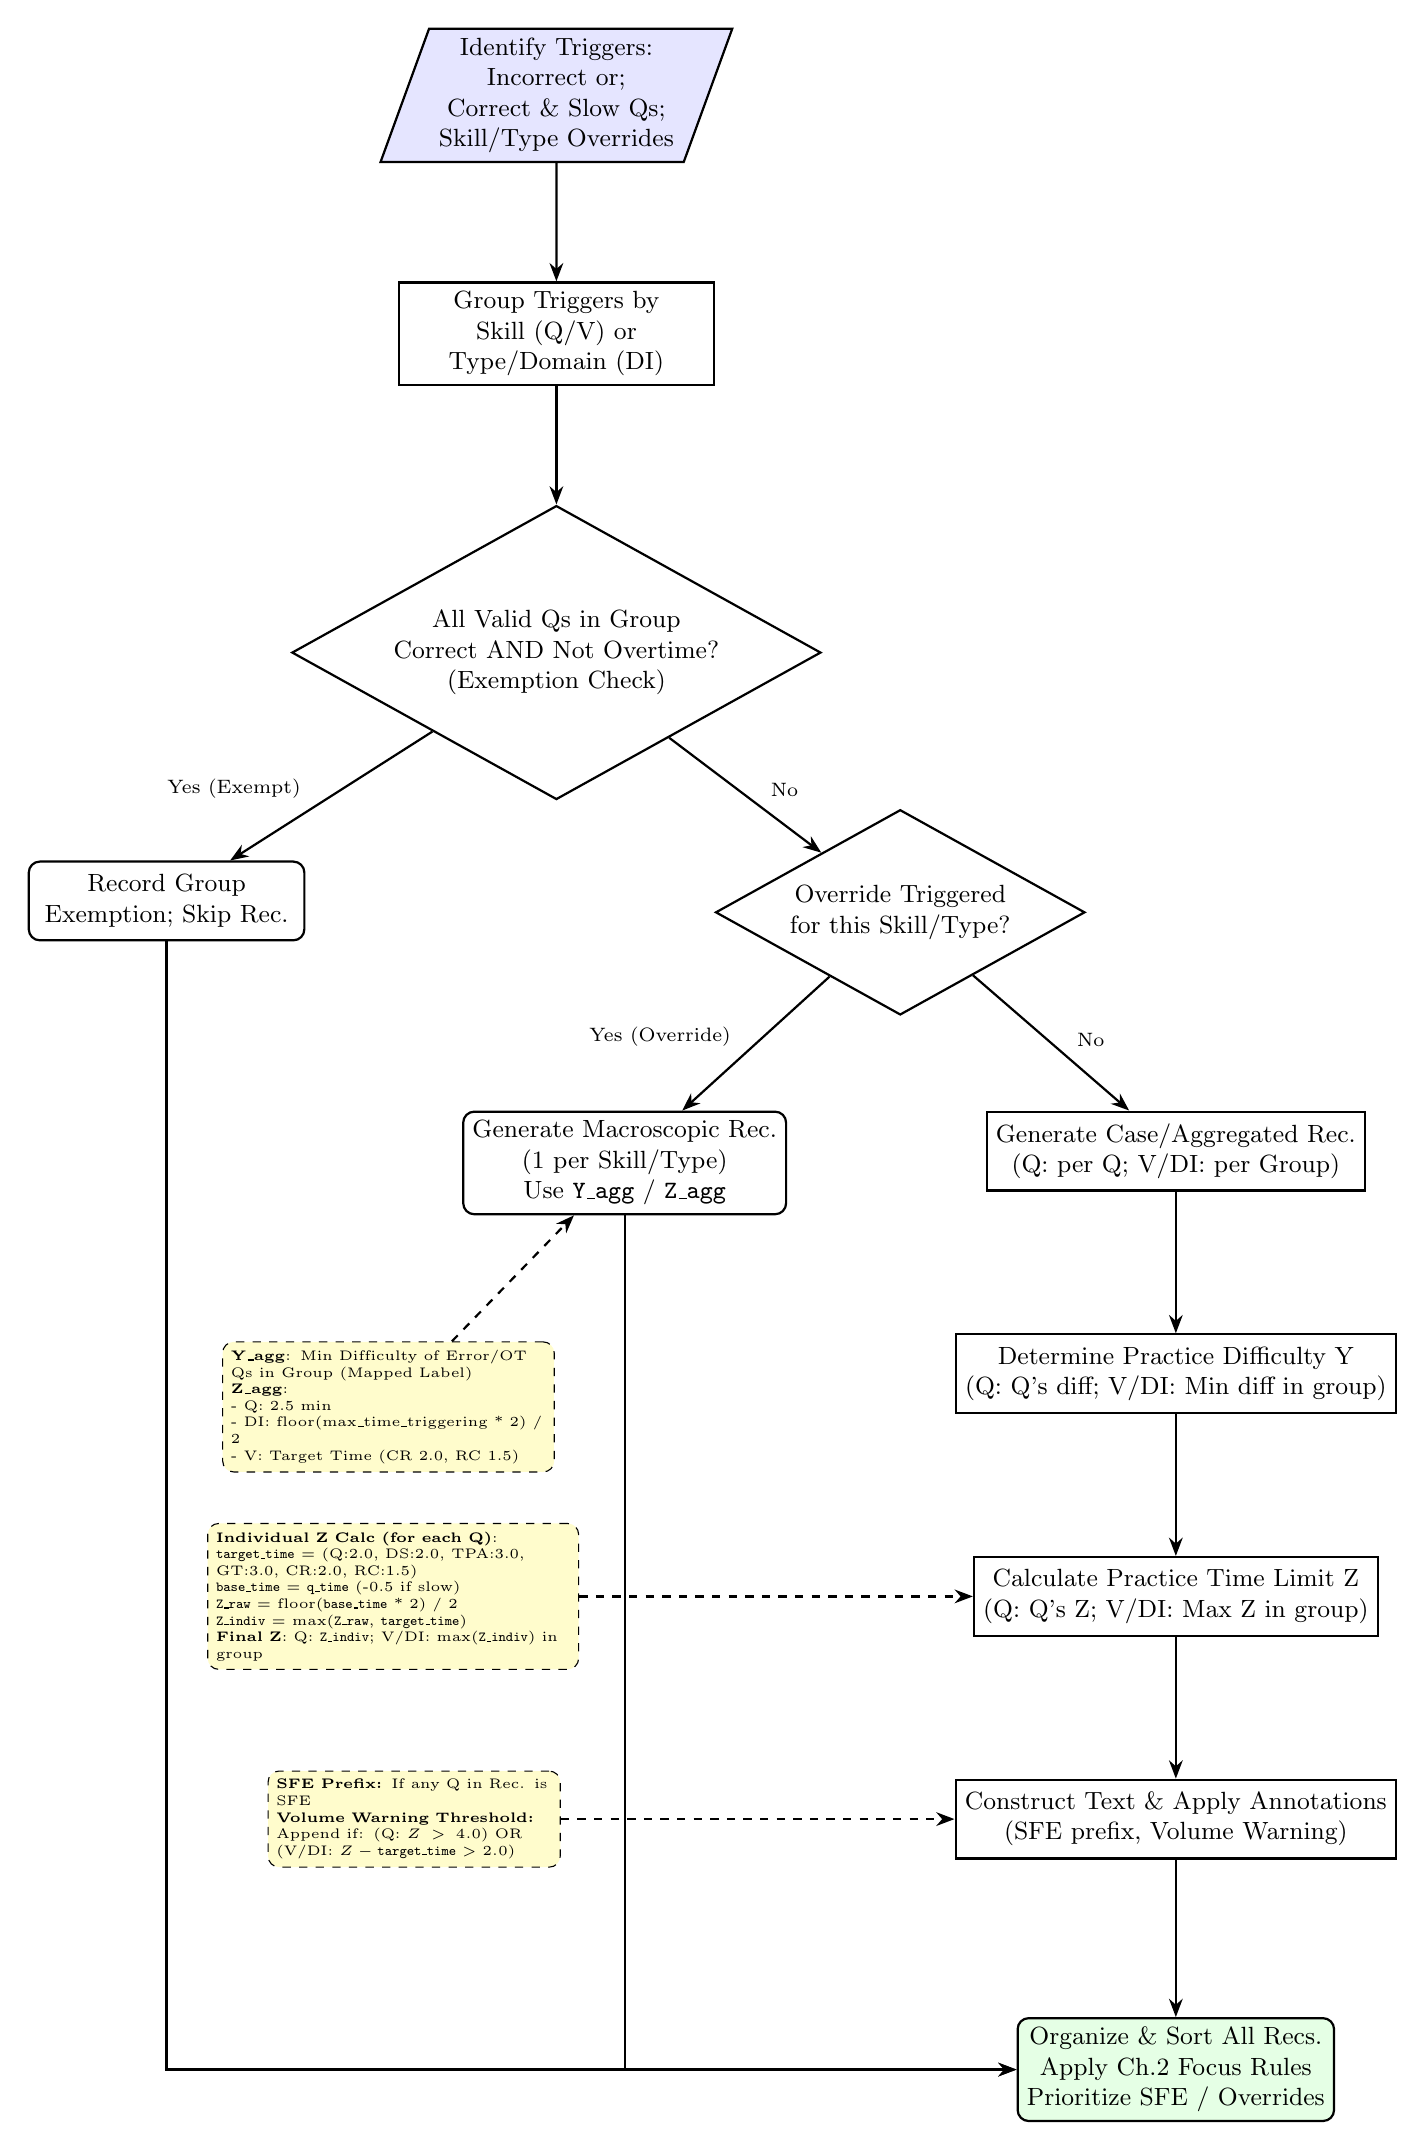
\begin{tikzpicture}[
    box/.style={rectangle, draw, rounded corners, minimum width=3.5cm, minimum height=1cm, text centered, font=\small, align=center, thick},
    decision/.style={diamond, draw, aspect=1.8, minimum width=4cm, minimum height=1.5cm, text centered, font=\small, align=center, thick},
    process/.style={rectangle, draw, minimum width=4cm, minimum height=1cm, text centered, font=\small, align=center, thick},
    data/.style={trapezium, draw, trapezium left angle=70, trapezium right angle=110, minimum width=3.2cm, minimum height=0.9cm, text centered, font=\small, fill=blue!10, thick},
    arrow/.style={-Stealth, thick}, % Changed to -Stealth
    param/.style={rectangle, draw, dashed, rounded corners, fill=yellow!20, font=\tiny, inner sep=3pt, align=left}, % Consistent param style
    node distance=1.5cm and 1cm % Adjusted node distance
]
% Input Data
% CORRECTED: Changed & to \&
\node[data, align=center, text width=3cm] (input) {Identify Triggers: Incorrect or; Correct \& Slow Qs; Skill/Type Overrides}; % Removed \\, added text width
% 注意:這裡直接把文字連起來,TikZ會根據 text width 自動換行。
% 你可能需要調整 3cm 這個寬度值。
% 也可以保留 \& 符號:
% \node[data, align=center, text width=3cm] (input) {Identify Triggers: Incorrect or; Correct & Slow Qs; Skill/Type Overrides};

% Categorization
\node[process, below=of input] (categorize) {Group Triggers by\\Skill (Q/V) or\\Type/Domain (DI)}; % More specific

% Iterate through each category/group
\node[decision, below=of categorize] (exemption) {All Valid Qs in Group\\Correct AND Not Overtime? \\ (Exemption Check)}; % Clarified text

\node[box, below left=of exemption, xshift=-0.5cm, yshift=-0.2cm] (exempt) {Record Group\\Exemption; Skip Rec.}; % Adjusted position and text
\node[decision, below right=of exemption, xshift=0.5cm,yshift=-0.2cm] (override) {Override Triggered\\for this Skill/Type?}; % Adjusted position and text

% Macroscopic Recommendation Path
\node[box, below = 1.2cm of override, xshift=-3.5cm] (macroscopic) {Generate Macroscopic Rec.\\(1 per Skill/Type)\\Use \texttt{Y\_agg} / \texttt{Z\_agg}}; % Adjusted position
\node[param, text width=4cm,
      below=of macroscopic, yshift=-0.1cm, xshift=-3cm]
  (macro_param) {
    \textbf{Y\_agg}: Min Difficulty of Error/OT Qs in Group (Mapped Label)\\
    \textbf{Z\_agg}:\\
    - Q: 2.5 min\\
    - DI: floor(max\_time\_triggering * 2) / 2\\
    - V: Target Time (CR 2.0, RC 1.5)
  };
\draw[arrow, dashed] (macro_param) -- (macroscopic);

% Case-Specific / Aggregated Recommendation Path
\node[process, below = 1.2cm of override, xshift=3.5cm] (case_gen) {Generate Case/Aggregated Rec.\\(Q: per Q; V/DI: per Group)}; % Adjusted position, clarified logic

\node[process, below=of case_gen, yshift=-0.3cm] (calc_y) {Determine Practice Difficulty Y\\(Q: Q's diff; V/DI: Min diff in group)}; % Clarified logic

\node[process, below=of calc_y, yshift=-0.3cm] (calc_z) {Calculate Practice Time Limit Z\\(Q: Q's Z; V/DI: Max Z in group)}; % Clarified logic
\node[param, text width=4.5cm,
      left=of calc_z, xshift=-4cm]
  (z_calc_detail) {
    \textbf{Individual Z Calc (for each Q)}:\\
    \texttt{target\_time} = (Q:2.0, DS:2.0, TPA:3.0, GT:3.0, CR:2.0, RC:1.5)\\
    \texttt{base\_time} = \texttt{q\_time} (-0.5 if slow)\\
    \texttt{Z\_raw} = floor(\texttt{base\_time} * 2) / 2\\
    \texttt{Z\_indiv} = max(\texttt{Z\_raw}, \texttt{target\_time}) \\
    \textbf{Final Z}: Q: \texttt{Z\_indiv}; V/DI: max(\texttt{Z\_indiv}) in group
};
\draw[arrow, dashed] (z_calc_detail) -- (calc_z);


\node[process, below=of calc_z, yshift=-0.3cm, align=center] (annotation) {Construct Text \& Apply Annotations\\(SFE prefix, Volume Warning)}; % Added text construction step

% CORRECTED: Added $ signs around >
\node[param, text width=3.5cm,
      left=of annotation, xshift=-4cm]
  (anno_param) {
    \textbf{SFE Prefix:} If any Q in Rec. is SFE\\
    \textbf{Volume Warning Threshold:}\\
    Append if: (Q: $Z > 4.0$) OR (V/DI: $Z - \texttt{target\_time} > 2.0$)
};
\draw[arrow, dashed] (anno_param) -- (annotation);


% Final Output
\node[box, below=of annotation, fill=green!10, yshift=-0.5cm] (organize) {Organize \& Sort All Recs.\\Apply Ch.2 Focus Rules\\Prioritize SFE / Overrides}; % Clarified sorting/focus

% Arrow Connections
\draw[arrow] (input) -- (categorize);
\draw[arrow] (categorize) -- (exemption);
\draw[arrow] (exemption) -- node[above left, font=\scriptsize, pos=0.6] {Yes (Exempt)} (exempt);
\draw[arrow] (exemption) -- node[above right, font=\scriptsize, pos=0.6] {No} (override);
\draw[arrow] (override) -- node[above left, font=\scriptsize, pos=0.6] {Yes (Override)} (macroscopic);
\draw[arrow] (override) -- node[above right, font=\scriptsize, pos=0.6] {No} (case_gen);
\draw[arrow] (case_gen) -- (calc_y);
\draw[arrow] (calc_y) -- (calc_z);
\draw[arrow] (calc_z) -- (annotation);
\draw[arrow] (annotation) -- (organize);
\draw[arrow] (exempt) |- (organize); % Connect exempt path to final output
\draw[arrow] (macroscopic) |- (organize); % Connect macroscopic path to final output

\end{tikzpicture}
}
\vspace{\baselineskip}
\caption{Flowchart for Chapter 7 Logic: Practice Recommendation Generation}
\label{fig:chapter7_logic}
\end{figure}
% ***** END OF FIGURE CODE *****

\subsection{Chapter 8: Diagnostic Summary and Subsequent Actions}

\textbf{Objective:} Synthesize all analysis findings and recommendations into a comprehensive, easily understandable report for the student, \textbf{using exclusively natural language}.

\textbf{Report Structure and Content Synthesis:}
\begin{enumerate}
    \item \textbf{Opening Summary:} This initial section synthesizes key findings from Chapter 1, including: the assessed \texttt{time\_pressure} status (described naturally, e.g., "significant time pressure was likely experienced"), total time usage relative to the limit, and whether any data was deemed invalid due to end-section rushing (e.g., "analysis excludes X questions answered hastily at the end under pressure"). \textbf{For DI sections}, include MSR group timing assessment and reading efficiency evaluation.
    \item \textbf{Performance Overview:} Summarizes Chapter 2 results descriptively: Relative performance across key dimensions (Q: 'Real' vs. 'Pure'; DI: 'Math Related' vs. 'Non-Math Related', types 'DS', 'TPA', 'GT'; V: Skill performance, 'CR' vs. 'RC') and difficulty levels (e.g., "Errors were concentrated in the High difficulty range," "Performance on 'Math Related' DI questions was significantly weaker than 'Non-Math Related'"). Mention reading time assessment for V if flagged. \textbf{For DI}, specifically address MSR group performance and reading efficiency patterns.
    \item \textbf{Core Problem Diagnosis:} Translates Chapter 3 findings into narrative form: Describes primary error patterns identified (e.g., "A tendency towards calculation errors in Pure Quant questions was observed," "Difficulties in interpreting complex graph relationships under time pressure were noted in GT questions," "Reading comprehension challenges in MSR passages affected subsequent question accuracy," "Logical flaws in evaluating assumptions were apparent in CR questions"). \textbf{Crucially highlights SFE findings} using descriptive language (e.g., "Particular attention is needed for errors occurring on questions below your typical mastery level in [Skill/Type], suggesting instability in applying fundamental concepts."). \textbf{Includes MSR-specific time issues for DI} if detected, with detailed reading strategy analysis.
    \item \textbf{Pattern Observation:} Integrates Chapter 5 alerts: Notes risks associated with early-stage rapid responses or potential carelessness if the \texttt{carelessness\_issue} flag was triggered (e.g., "A pattern of rapid, incorrect answers suggests that focusing on accuracy over speed may be beneficial"). \textbf{For DI}, includes MSR reading pattern observations and time allocation efficiency notes.
    \item \textbf{Foundational Consolidation Advisory:} Explicitly states which skills/types require systematic foundational work based on Chapter 6 override triggers (e.g., "Systematic review and practice of the fundamentals for [Skill/Type] is recommended due to overall performance patterns"). \textbf{For DI}, includes MSR reading strategy consolidation recommendations when applicable.
    \item \textbf{Practice Plan Presentation:} Presents the full, organized list of recommendations generated in Chapter 7, ensuring clarity and including all annotations (priority, volume alerts, focus rules, exemptions, MSR-specific guidance) in natural language descriptions within the recommendation text itself.
    \item \textbf{Guidance for Subsequent Actions:} Provides actionable next steps:
    \begin{itemize}
        \item \textbf{Guiding Reflection Questions:} Poses targeted, open-ended questions based on the specific diagnoses to prompt student self-assessment. \textbf{For DI}, incorporates MSR-specific questions about reading approach, note-taking strategy, and time allocation between reading and questions.
        \item \textbf{Secondary Evidence Review Suggestion:} Explains \textit{when} (e.g., uncertain recall, need pattern confirmation, MSR strategy unclear) and \textit{how} (e.g., review recent logs, focus on specific error types, analyze MSR reading habits) to use past practice data.
        \item \textbf{Qualitative Analysis Suggestion:} Explains \textit{when} (e.g., root cause remains unclear after other steps, MSR reading strategy needs refinement) and \textit{how} (e.g., provide detailed walkthroughs for specific problem types, MSR reading technique demonstration) to engage in deeper analysis, potentially with an advisor.
    \end{itemize}
\end{enumerate}

\textbf{Core Constraint Adherence:} The implementation generating this chapter\'s output must rigorously avoid exposing internal variable names (e.g., \texttt{time\_pressure}, \texttt{is\_invalid}, \texttt{special\_focus\_error}, \texttt{msr\_group\_id}), specific performance flags, numerical thresholds, or calculation details. All findings must be translated into clear, easily understandable, descriptive prose suitable for the end-user (student). \textbf{DI-specific technical details} such as MSR group algorithms, reading time calculations, and statistical thresholds should be abstracted into user-friendly reading strategy guidance.

\textbf{Implementation Context:} This is typically handled by a dedicated \texttt{generate\_report\_*} function that receives all computed metrics, flags, lists, and generated recommendation texts as arguments. It uses conditional statements (\texttt{if/else}) and formatted strings (\texttt{f-strings}) to assemble the report sections based on the presence and values of these inputs, ensuring adherence to the natural language constraint. \textbf{For DI sections}, special handling functions process MSR group data and convert technical timing analysis into readable reading strategy recommendations.

\textbf{Rationale:} Provides a holistic, actionable summary translating complex quantitative diagnostics and parameterized recommendations into clear, user-friendly insights and next steps, maximizing the practical value of the analysis for the student. The natural language presentation ensures accessibility while maintaining the analytical rigor of the underlying diagnostic framework. \textbf{For DI sections}, this includes making MSR reading strategy analysis accessible and actionable for students.

\subsection{Illustrative Example: Simplified Question Journey}

To illustrate how the framework processes a single question, consider this simplified hypothetical example for a Quant ('Pure') question:

\textbf{Input Data:}
\begin{itemize}
    \item \texttt{question\_id}: Q5
    \item \texttt{question\_time}: 3.2 min
    \item \texttt{is\_correct}: False
    \item \texttt{question\_difficulty}: 650
    \item \texttt{question\_position}: 10 (out of 21)
    \item \texttt{question\_type}: 'Pure'
    \item \texttt{question\_fundamental\_skill}: 'Algebra'
    \item (Assume \texttt{total\_test\_time} = 43 min, \texttt{max\_allowed\_time} = 45 min, implies \texttt{time\_pressure} = False based on Q/DI rule)
    \item (Assume \texttt{average\_time\_per\_type} for 'Pure' = 2.1 min)
    \item (Assume \texttt{max\_mastered\_difficulty} for 'Algebra' = 700)
\end{itemize}
\newpage
\textbf{Framework Steps Applied:}
\begin{enumerate}
    \item \textbf{Chapter 1 (Validity/Overtime):}
        \begin{itemize}
            \item \texttt{time\_pressure} is False.
            \item \texttt{question\_position} is not in the last third, and \texttt{question\_time} $>$ 1.0 min $\rightarrow$ \texttt{is\_invalid} = False. (Data is valid). % CORRECTED: Added $ sign
            \item The \texttt{overtime\_threshold} for Q (no pressure) is 3.0 min. Since 3.2 min $>$ 3.0 min $\rightarrow$ \texttt{overtime} = True. % CORRECTED: Added $ sign
        \end{itemize}
    \item \textbf{Chapter 2 (Performance - Context):} This question contributes to the overall metrics for 'Pure' type, 'Algebra' skill, and the corresponding difficulty band (e.g., "Medium / 605+").
    \item \textbf{Chapter 3 (Root Cause):}
        \begin{itemize}
            \item Time Classification: 3.2 min is not $<$ (2.1 * 0.75) $\rightarrow$ \texttt{is\_relatively\_fast} = False. Since \texttt{overtime} is True $\rightarrow$ \texttt{is\_slow} = True. % CORRECTED: Added $ sign
            \item SFE Check: \texttt{is\_correct} is False, and \texttt{question\_difficulty} (650) $<$ \texttt{max\_mastered\_difficulty} (700) $\rightarrow$ \texttt{special\_focus\_error} = True. % CORRECTED: Added $ sign
            \item Scenario: Slow \& Wrong \& SFE.
        \end{itemize}
    \item \textbf{Chapter 6 (Coverage - Check):} Check if 'Algebra' skill has \texttt{error\_rate} or \texttt{overtime\_rate} $>$ 50\%. (Assume for this example it does not $\rightarrow$ \texttt{skill\_override\_triggered}['Algebra'] = False). % CORRECTED: Added $ sign
    \item \textbf{Chapter 7 (Recommendation):}
        \begin{enumerate}
            \item Trigger: Incorrect question (Q5).
            \item Exemption/Override: Not exempt (based on other Algebra questions) and not overridden.
            \item Y (Difficulty): Map 650 to label (e.g., "Medium / 605+").
            \item Z (Time): \texttt{is\_slow} is True. \texttt{base\_time} = 3.2 - 0.5 = 2.7. \texttt{Z\_raw} = floor(2.7 * 2) / 2 = floor(5.4) / 2 = 5.0 / 2 = 2.5. \texttt{target\_time} for Q is 2.0. \texttt{Z} = max(2.5, 2.0) = 2.5 min.
            \item Annotation: Prepend "*Fundamental mastery potentially unstable:* Practice Algebra ('Pure') problems at Medium / 605+ difficulty, starting with a 2.5 min time limit (target 2.0 min)."
        \end{enumerate}
\end{enumerate}
This example shows the flow from raw data through flagging (overtime, SFE) to a specific, annotated recommendation based on the framework's rules.

\subsection{Implementation Details}

The unified diagnostic framework described herein has been implemented as a set of Python scripts (\texttt{gmat\_q\_analyzer.py}, \texttt{gmat\_di\_analyzer.py}, \texttt{gmat\_v\_analyzer.py}), one for each GMAT section. The development followed an iterative process involving requirements analysis based on the methodological documents (\texttt{en-gmat-\*.md}), coding, testing with sample datasets (\texttt{testset-\*.csv}), debugging, and refinement based on analysis outcomes and evolving reporting requirements.

\textbf{Core Technologies:}
\begin{itemize}
    \item \textbf{Python:} The primary programming language.
    \item \textbf{Pandas:} Extensively used for data manipulation, including reading CSV files, data cleaning (handling missing values, type conversion), filtering, grouping, aggregation, and time-series operations where applicable. DataFrame structures are central to storing and processing the per-question data and analytical results.
    \item \textbf{NumPy:} Utilized for numerical operations, handling potential \texttt{NaN} values, and creating placeholder data structures (e.g., spacer rows using \texttt{np.nan}).
    \item \textbf{Argparse:} Employed for command-line argument parsing, allowing users to specify input/output file paths and optional flags (e.g., overriding \texttt{time\_pressure} status).
\end{itemize}

\textbf{Development Challenges \& Solutions:}
\begin{itemize}
    \item \textbf{Environment \& Dependencies:} Initial challenges included resolving Python interpreter path issues and managing dependencies (\texttt{pandas}, \texttt{numpy}). The use of Python virtual environments (\texttt{venv}) was adopted to ensure consistent and isolated execution environments, addressing \texttt{externally-managed-environment} errors related to PEP 668.
    \item \textbf{Data Inconsistencies:} Handling variations in input CSV formats, such as extra commas in headers or differing column names (e.g., \texttt{V\_b}, \texttt{DI\_b} vs. a consistent \texttt{question\_difficulty}), required robust parsing logic (e.g., using \texttt{usecols} in \texttt{pd.read\_csv}, dynamic column renaming). Encoding issues were addressed by attempting multiple common encodings (\texttt{utf-8}, \texttt{gbk}, \texttt{cp950}).
    \item \textbf{Logic Implementation:} Translating the sometimes complex, multi-conditional logic from the markdown documents into precise code required careful structuring, particularly for overtime calculations, SFE detection, and recommendation generation involving multiple interacting rules (override, exemption, focus). Helper functions were created to encapsulate reusable logic (e.g., difficulty mapping, safe division, Z-time calculation, MSR/RC group processing).
    \item \textbf{Pandas Operations:} Specific \texttt{pandas} operations occasionally led to errors (e.g., ambiguity in boolean operations on DataFrames, errors during DataFrame initialization with specific structures like \texttt{[[]] * n}), necessitating refactoring to use element-wise operations or more robust initialization methods (\texttt{pd.DataFrame(np.nan, ...)}).
    \item \textbf{Evolving Requirements:} The most significant evolution was the increasing demand for report granularity. Initial implementations produced summary-level reports, but later iterations required significant refactoring to generate detailed, per-question diagnostics, actions, reflections, and evidence prompts, necessitating the creation of \texttt{get\_detailed\_diagnosis\_*} functions and modifications to the main analysis loop and report generation logic across all three scripts.
    \item \textbf{Debugging:} Identifying the root cause of errors often involved tracing data flow through the DataFrame, checking intermediate values, and verifying that conditional logic correctly handled edge cases (e.g., division by zero, empty data subsets after filtering). \texttt{NameError} and \texttt{KeyError} issues were common during refactoring, requiring careful checking of variable scope and dictionary key handling.
\end{itemize}

\textbf{Output Data Format (Annotated CSV):}
In addition to the natural language summary report, the Python scripts generate an output CSV file (e.g., \texttt{testset-q-analyzed.csv}). This file contains all the original input data plus several new columns representing the diagnostic flags calculated during the analysis. Key added columns include:

\begin{itemize}
    \item \texttt{difficulty\_label}: The standardized difficulty category (e.g., "Medium / 605+").
    \item \texttt{time\_pressure}: Boolean flag indicating if overall time pressure was detected (Chapter 1).
    \item \texttt{is\_invalid}: Boolean flag indicating if the question data was excluded due to extreme rushing under time pressure (Chapter 1).
    \item \texttt{overtime} (or variants like \texttt{group\_overtime}): Boolean flag indicating if the question (or group) exceeded the calculated overtime threshold based on the *filtered* data (Chapter 1).
    \item \texttt{is\_relatively\_fast}: Boolean flag indicating if the question was answered significantly faster than the average for its type (Chapter 3).
    \item \texttt{is\_slow}: Boolean flag, essentially mirroring the \texttt{overtime} flag for consistency in time classification (Chapter 3).
    \item \texttt{max\_mastered\_difficulty}: The highest difficulty level mastered within the relevant skill/type category based on correct answers (Chapter 3).
    \item \texttt{special\_focus\_error}: A Boolean indicator signifying an error made on a question possessing a difficulty level inferior to the user's attained \texttt{max\_mastered\_difficulty} within that specific subject category (as specified in Chapter 3).
    \item \texttt{skill\_override\_triggered} / \texttt{override\_triggered}: Boolean flag indicating if a coverage rule was triggered for the question's skill/type (Chapter 6).
    \item \texttt{Recommendation\_Y}: The suggested practice difficulty level (String label).
    \item \texttt{Recommendation\_Z}: The suggested starting practice time limit (Numeric, minutes).
    \item \texttt{Diagnostic\_Notes}: Text field containing generated diagnostic comments or recommendation details.
\end{itemize}
This annotated CSV allows for detailed review and further analysis of the framework's per-question conclusions.

\textbf{Current State:} The resulting Python scripts represent functional implementations of the diagnostic framework. They successfully ingest section-specific GMAT data, apply the complex analytical logic outlined in Chapters 0-7, handle various data edge cases, and produce detailed output CSV files containing both per-question diagnostic flags and a comprehensive, natural-language summary report adhering to the structure of Chapter 8. The scripts are designed to be run from the command line, providing a practical tool for automated GMAT performance analysis.

\section{Conclusion}

The primary value of this framework, as detailed in this technical report, lies in its systematic and unified approach to formalizing the complex process of GMAT performance diagnosis across multiple sections. It provides a transparent, structured, and potentially automatable methodology moving beyond simple metrics.

As documentation focused on the framework's design, readers should note its current limitations. The specific parameter values used in the implementation represent informed heuristics derived from initial analysis and expert consultation, rather than statistically optimized values derived from large-scale empirical validation. While preliminary comparisons to expert analysis are encouraging, rigorous validation of the framework's diagnostic accuracy and effectiveness remains a crucial next step for future development.

The unified GMAT diagnostic framework presented offers a systematic, multi-faceted approach to analyzing student performance across the Quantitative, Data Insights, and Verbal sections. By adhering to a consistent chapter-based structure while accommodating section-specific nuances through parameterized logic and tailored analyses, the framework moves beyond superficial score reporting to identify root causes of errors and inefficiencies. Key strengths include:

\begin{itemize}
    \item \textbf{Comprehensive Scope:} Addresses time management, data validity, accuracy, efficiency, behavioral patterns, and foundational knowledge across all scored sections.
    \item \textbf{Depth of Analysis:} Employs concepts like relative time performance, \texttt{special\_focus\_error} detection, and coverage rules to provide nuanced diagnoses based on operationalized parameters.
    \item \textbf{Actionable Output:} Generates personalized practice plans with specific difficulty (\texttt{Y}/\texttt{Y\_agg}) and time (\texttt{Z}/\texttt{Z\_agg}) parameters, alongside structured guidance for self-reflection and further analysis.
    \item \textbf{Standardization \& Adaptability:} Provides a consistent analytical process applicable to Q, DI, and V, ensuring comparable insights while respecting the unique demands of each section, as evidenced by the successful implementation across three distinct Python modules.
\end{itemize}

This framework, validated through empirical testing and refinement, empowers students and instructors with detailed, data-driven insights, facilitating more targeted preparation and ultimately aiming for improved GMAT performance.

\section{Future Directions}

Building upon the established framework and its current implementation, several avenues for future development and application are envisioned:

\begin{enumerate}
    \item \textbf{Web-Based Implementation:} To enhance accessibility and utility, the diagnostic framework is planned for implementation as an automated, user-facing tool integrated into a web platform. This would allow students to upload their score data (e.g., via CSV or potentially through direct API integration if available) and receive instant, standardized diagnostic reports through a user-friendly interface.
   \item \textbf{Rigorous Parameter Optimization and Validation:} Beyond initial heuristics, future work involves rigorously validating and optimizing framework parameters (e.g., time thresholds, speed factors, SFE sensitivity, coverage rules) and predictive accuracy. Hyperparameter optimization methods like Grid Search will be used on larger student datasets to find parameter sets maximizing concordance between the framework's diagnoses and validated metrics or expert assessments, enhancing diagnostic and predictive effectiveness.
    \item \textbf{Integration of Qualitative Feedback:} Explore methods to integrate qualitative student feedback (e.g., self-reported reasons for errors, confidence levels) directly into the diagnostic process, potentially refining the root cause analysis beyond purely quantitative data.
    \item \textbf{Longitudinal Analysis:} Extend the framework to analyze performance trends over multiple test administrations or practice sessions for a single student, identifying patterns of improvement or persistent weaknesses.
\end{enumerate}
\newpage
% Use \appendix command for proper appendix formatting
\appendix
% \newpage % Start Appendix on a new page - \appendix command might handle this
\section*{Appendix A: Diagnostic Parameter Tags and Descriptions} % Use section* for unnumbered section

\vspace{1em} % Add some vertical space before the table

% --- Start of the longtable with single column format ---
% Remember to have \usepackage{longtable} in your preamble
{ % Start group to limit the scope of \arraystretch
\renewcommand{\arraystretch}{1.1} % Spacing for better readability

\begin{longtable}{|p{0.95\textwidth}|} % Single column format using most of page width

% --- Header Definitions ---
\caption{Diagnostic Parameter Tags and Descriptions}% Add caption if needed
\label{tab:diagnostic_tags}\\ % Add label if needed for referencing
\hline % Top line for the first page header
\textbf{Diagnostic Parameter Tags and Descriptions} \\ % Header content
\hline % Line below header content
\endfirsthead % Marks the end of the header for the first page

\hline % Top line for continuation page header
\tablename\ \thetable{} -- \textit{Continued from previous page} \\ % Title for continued pages
\hline % Line below the continued title
\endhead % Marks the end of the header for continuation pages

\hline % Line above the footer on pages before the last
\textit{Continued on next page} \\ % Footer content for pages before the last
\endfoot % Marks the end of the footer for pages before the last

\hline % Bottom line for the table on the last page
\endlastfoot % Marks the end of the footer for the last page

% --- Table Content Starts Here ---
\hline
\textbf{Reading / Comprehension / Interpretation} \\
\hline
\texttt{Q\_READING\_COMPREHENSION\_ERROR} \\
Q Reading: Difficulty understanding word problem text (Real Context) \\
\hline
\texttt{Q\_PROBLEM\_UNDERSTANDING\_ERROR} \\
Q Problem Understanding: Misinterpretation of question requirements/logic \\
\hline
\texttt{DI\_READING\_COMPREHENSION\_ERROR} \\
DI Reading Comprehension: Error/Difficulty understanding text (Math/Non-Math) \\
\hline
\texttt{DI\_GRAPH\_TABLE\_INTERPRETATION\_ERROR} \\
DI Graph/Table Interpretation: Error/Difficulty interpreting visual data \\
\hline
\texttt{DI\_MSR\_READING\_COMPREHENSION\_BARRIER} \\
DI MSR Reading Barrier: Excessive overall reading time affecting group performance \\
\hline
\textbf{Concept / Logic Application} \\
\hline
\texttt{Q\_CONCEPT\_APPLICATION\_ERROR} \\
Q Concept Application: Error applying mathematical concepts/formulas \\
\hline
\texttt{DI\_CONCEPT\_APPLICATION\_ERROR} \\
DI Concept Application (Math): Error applying mathematical concepts/formulas \\
\hline
\texttt{DI\_LOGICAL\_REASONING\_ERROR} \\
DI Logical Reasoning (Non-Math): Error in inherent logical reasoning/judgment \\
\hline
\textbf{Data Handling / Calculation / Location} \\
\hline
\texttt{Q\_CALCULATION\_ERROR} \\
Q Calculation: Error in mathematical computation \\
\hline
\texttt{DI\_DATA\_EXTRACTION\_ERROR} \\
DI Data Extraction (GT): Error extracting data from graphs/tables \\
\hline
\texttt{DI\_INFORMATION\_EXTRACTION\_INFERENCE\_ERROR} \\
DI Info Extraction/Inference (GT/MSR Non-Math): Error locating/inferring information \\
\hline
\texttt{DI\_CALCULATION\_ERROR} \\
DI Calculation: Error in mathematical computation \\
\hline
\texttt{DI\_MSR\_TIME\_ALLOCATION\_ISSUE} \\
DI MSR Time Allocation: Inefficient time distribution between reading and questions \\
\hline
\textbf{Section/Type Specific (MSR - DI Only)} \\
\hline
\texttt{DI\_MULTI\_SOURCE\_INTEGRATION\_ERROR} \\
DI Multi-Source Integration (MSR): Error integrating information across multiple sources \\
\hline
\texttt{DI\_MSR\_READING\_STRATEGY\_INEFFICIENCY} \\
DI MSR Reading Strategy: Inefficient reading approach for multi-source materials \\
\hline
\texttt{DI\_MSR\_GROUP\_TIMING\_MANAGEMENT\_ERROR} \\
DI MSR Group Timing Management: Poor time management across MSR question groups \\
\hline
\texttt{DI\_QUESTION\_TYPE\_SPECIFIC\_ERROR} \\
DI Question Type Specific Error (e.g., DS, TPA, GT specific weaknesses) \\
\hline
\texttt{DI\_MSR\_READING\_DEPTH\_VS\_SPEED\_IMBALANCE} \\
DI MSR Reading: Imbalance between reading depth and speed requirements \\
\hline
\textbf{Critical Reasoning (CR) - Verbal} \\
\hline
\textit{CR Stem Understanding Errors} \\
\hline
\texttt{CR\_STEM\_UNDERSTANDING\_ERROR\_QUESTION\_REQUIREMENT\_GRASP} \\
CR Stem Understanding Error: Misinterpretation of question requirements \\
\hline
\texttt{CR\_STEM\_UNDERSTANDING\_ERROR\_VOCAB} \\
CR Stem Understanding Error: Vocabulary issues in stem \\
\hline
\texttt{CR\_STEM\_UNDERSTANDING\_ERROR\_SYNTAX} \\
CR Stem Understanding Error: Syntactical complexity in stem \\
\hline
\texttt{CR\_STEM\_UNDERSTANDING\_ERROR\_LOGIC} \\
CR Stem Understanding Error: Logical structure of stem misunderstood \\
\hline
\texttt{CR\_STEM\_UNDERSTANDING\_ERROR\_DOMAIN} \\
CR Stem Understanding Error: Domain-specific content in stem misunderstood \\
\hline
\textit{CR Reasoning Errors} \\
\hline
\texttt{CR\_REASONING\_ERROR\_LOGIC\_CHAIN\_ANALYSIS\_PREMISE\_CONCLUSION\_RELATIONSHIP} \\
CR Reasoning Error: Flawed analysis of premise-conclusion relationship \\
\hline
\texttt{CR\_REASONING\_ERROR\_ABSTRACT\_LOGIC\_TERMINOLOGY\_UNDERSTANDING} \\
CR Reasoning Error: Misunderstanding of abstract logic or terminology \\
\hline
\texttt{CR\_REASONING\_ERROR\_PREDICTION\_DIRECTION} \\
CR Reasoning Error: Incorrect prediction of answer direction \\
\hline
\texttt{CR\_REASONING\_ERROR\_CORE\_ISSUE\_IDENTIFICATION} \\
CR Reasoning Error: Failure to identify the core issue of the argument \\
\hline
\texttt{CR\_REASONING\_ERROR\_CHOICE\_RELEVANCE\_JUDGEMENT} \\
CR Reasoning Error: Incorrect judgment of answer choice relevance \\
\hline
\texttt{CR\_REASONING\_ERROR\_STRONG\_DISTRACTOR\_CHOICE\_CONFUSION} \\
CR Reasoning Error: Confusion caused by strong distractor choices \\
\hline
\textit{CR Choice Understanding Errors} \\
\hline
\texttt{CR\_CHOICE\_UNDERSTANDING\_ERROR\_VOCAB} \\
CR Choice Understanding Error: Vocabulary issues in answer choices \\
\hline
\texttt{CR\_CHOICE\_UNDERSTANDING\_ERROR\_SYNTAX} \\
CR Choice Understanding Error: Syntactical complexity in answer choices \\
\hline
\texttt{CR\_CHOICE\_UNDERSTANDING\_ERROR\_LOGIC} \\
CR Choice Understanding Error: Logical structure of answer choices misunderstood \\
\hline
\texttt{CR\_CHOICE\_UNDERSTANDING\_ERROR\_DOMAIN} \\
CR Choice Understanding Error: Domain-specific content in choices misunderstood \\
\hline
\textit{CR Specific Question Type Weakness} \\
\hline
\texttt{CR\_SPECIFIC\_QUESTION\_TYPE\_WEAKNESS\_NOTE\_TYPE} \\
CR Specific Question Type Weakness: (Type to be noted) \\
\hline
\textit{CR Stem Understanding Difficulties (Efficiency Issue / Slow Performance)} \\
\hline
\texttt{CR\_STEM\_UNDERSTANDING\_DIFFICULTY\_VOCAB} \\
CR Stem Understanding Difficulty: Vocabulary challenges in stem \\
\hline
\texttt{CR\_STEM\_UNDERSTANDING\_DIFFICULTY\_SYNTAX} \\
CR Stem Understanding Difficulty: Syntactical complexity in stem causing slowdown \\
\hline
\texttt{CR\_STEM\_UNDERSTANDING\_DIFFICULTY\_LOGIC} \\
CR Stem Understanding Difficulty: Logical structure of stem hard to grasp \\
\hline
\texttt{CR\_STEM\_UNDERSTANDING\_DIFFICULTY\_DOMAIN} \\
CR Stem Understanding Difficulty: Domain-specific content in stem hard to grasp \\
\hline
\textit{CR Reasoning Difficulties (Efficiency Issue / Slow Performance)} \\
\hline
\texttt{CR\_REASONING\_DIFFICULTY\_ABSTRACT\_LOGIC\_TERMINOLOGY\_UNDERSTANDING} \\
CR Reasoning Difficulty: Difficulty with abstract logic or terminology \\
\hline
\texttt{CR\_REASONING\_DIFFICULTY\_PREDICTION\_DIRECTION\_MISSING} \\
CR Reasoning Difficulty: Missing or slow prediction of answer direction \\
\hline
\texttt{CR\_REASONING\_DIFFICULTY\_CORE\_ISSUE\_IDENTIFICATION} \\
CR Reasoning Difficulty: Difficulty identifying the core issue of the argument \\
\hline
\texttt{CR\_REASONING\_DIFFICULTY\_CHOICE\_RELEVANCE\_JUDGEMENT} \\
CR Reasoning Difficulty: Difficulty judging answer choice relevance \\
\hline
\texttt{CR\_REASONING\_DIFFICULTY\_STRONG\_DISTRACTOR\_CHOICE\_ANALYSIS} \\
CR Reasoning Difficulty: Difficulty analyzing strong distractor choices \\
\hline
\textit{CR Choice Understanding Difficulties (Efficiency Issue / Slow Performance)} \\
\hline
\texttt{CR\_CHOICE\_UNDERSTANDING\_DIFFICULTY\_VOCAB} \\
CR Choice Understanding Difficulty: Vocabulary challenges in answer choices \\
\hline
\texttt{CR\_CHOICE\_UNDERSTANDING\_DIFFICULTY\_SYNTAX} \\
CR Choice Understanding Difficulty: Syntactical complexity in choices causing slowdown \\
\hline
\texttt{CR\_CHOICE\_UNDERSTANDING\_DIFFICULTY\_LOGIC} \\
CR Choice Understanding Difficulty: Logical structure of choices hard to grasp \\
\hline
\texttt{CR\_CHOICE\_UNDERSTANDING\_DIFFICULTY\_DOMAIN} \\
CR Choice Understanding Difficulty: Domain-specific content in choices hard to grasp \\
\hline
\textbf{Reading Comprehension (RC) - Verbal} \\
\hline
\textit{RC Reading Comprehension Errors} \\
\hline
\texttt{RC\_READING\_COMPREHENSION\_ERROR\_VOCAB} \\
RC Reading Comprehension Error: Vocabulary misunderstanding \\
\hline
\texttt{RC\_READING\_COMPREHENSION\_ERROR\_LONG\_DIFFICULT\_SENTENCE\_ANALYSIS} \\
RC Reading Comprehension Error: Incorrect analysis of long/difficult sentences \\
\hline
\texttt{RC\_READING\_COMPREHENSION\_ERROR\_PASSAGE\_STRUCTURE} \\
RC Reading Comprehension Error: Misunderstanding of passage structure \\
\hline
\texttt{RC\_READING\_COMPREHENSION\_ERROR\_KEY\_INFO\_LOCATION\_UNDERSTANDING} \\
RC Reading Comprehension Error: Incorrect location or understanding of key information \\
\hline
\textit{RC Question Understanding Errors} \\
\hline
\texttt{RC\_QUESTION\_UNDERSTANDING\_ERROR\_FOCUS\_POINT} \\
RC Question Understanding Error: Misinterpretation of the question's focus point \\
\hline
\textit{RC Location Skill Errors} \\
\hline
\texttt{RC\_LOCATION\_SKILL\_ERROR\_LOCATION} \\
RC Location Skill Error: Incorrect location of information in the passage \\
\hline
\textit{RC Reasoning Errors} \\
\hline
\texttt{RC\_REASONING\_ERROR\_INFERENCE} \\
RC Reasoning Error: Flawed inference from the passage text \\
\hline
\textit{RC Choice Analysis Errors} \\
\hline
\texttt{RC\_CHOICE\_ANALYSIS\_ERROR\_VOCAB} \\
RC Choice Analysis Error: Vocabulary issues in answer choices \\
\hline
\texttt{RC\_CHOICE\_ANALYSIS\_ERROR\_SYNTAX} \\
RC Choice Analysis Error: Syntactical complexity in answer choices \\
\hline
\texttt{RC\_CHOICE\_ANALYSIS\_ERROR\_LOGIC} \\
RC Choice Analysis Error: Logical structure of answer choices misunderstood \\
\hline
\texttt{RC\_CHOICE\_ANALYSIS\_ERROR\_DOMAIN} \\
RC Choice Analysis Error: Domain-specific content in choices misunderstood \\
\hline
\texttt{RC\_CHOICE\_ANALYSIS\_ERROR\_RELEVANCE\_JUDGEMENT} \\
RC Choice Analysis Error: Incorrect judgment of answer choice relevance \\
\hline
\texttt{RC\_CHOICE\_ANALYSIS\_ERROR\_STRONG\_DISTRACTOR\_CONFUSION} \\
RC Choice Analysis Error: Confusion caused by strong distractor choices \\
\hline
\textit{RC Method Errors} \\
\hline
\texttt{RC\_METHOD\_ERROR\_SPECIFIC\_QUESTION\_TYPE\_HANDLING} \\
RC Method Error: Incorrect handling of specific question types \\
\hline
\textit{RC Reading Comprehension Difficulties (Efficiency Issue / Slow Performance)} \\
\hline
\texttt{RC\_READING\_COMPREHENSION\_DIFFICULTY\_VOCAB\_BOTTLENECK} \\
RC Reading Comprehension Difficulty: Vocabulary bottleneck \\
\hline
\texttt{RC\_READING\_COMPREHENSION\_DIFFICULTY\_LONG\_DIFFICULT\_SENTENCE\_ANALYSIS} \\
RC Reading Comprehension Difficulty: Difficulty analyzing long/difficult sentences \\
\hline
\texttt{RC\_READING\_COMPREHENSION\_DIFFICULTY\_PASSAGE\_STRUCTURE\_GRASP\_UNCLEAR} \\
RC Reading Comprehension Difficulty: Unclear grasp of passage structure \\
\hline
\texttt{RC\_READING\_COMPREHENSION\_DIFFICULTY\_SPECIFIC\_DOMAIN\_BACKGROUND\_KNOWLEDGE\_LACK} \\
RC Reading Comprehension Difficulty: Lack of specific domain background knowledge \\
\hline
\textit{RC Question Understanding Difficulties (Efficiency Issue / Slow Performance)} \\
\hline
\texttt{RC\_QUESTION\_UNDERSTANDING\_DIFFICULTY\_FOCUS\_POINT\_GRASP} \\
RC Question Understanding Difficulty: Difficulty grasping the question's focus point \\
\hline
\textit{RC Location Skill Difficulties (Efficiency Issue / Slow Performance)} \\
\hline
\texttt{RC\_LOCATION\_SKILL\_DIFFICULTY\_INEFFICIENCY} \\
RC Location Skill Difficulty: Inefficient location of information \\
\hline
\textit{RC Reasoning Difficulties (Efficiency Issue / Slow Performance)} \\
\hline
\texttt{RC\_REASONING\_DIFFICULTY\_INFERENCE\_SPEED\_SLOW} \\
RC Reasoning Difficulty: Slow inference speed \\
\hline
\textit{RC Choice Analysis Difficulties (Efficiency Issue / Slow Performance)} \\
\hline
\texttt{RC\_CHOICE\_ANALYSIS\_DIFFICULTY\_VOCAB} \\
RC Choice Analysis Difficulty: Vocabulary challenges in answer choices \\
\hline
\texttt{RC\_CHOICE\_ANALYSIS\_DIFFICULTY\_SYNTAX} \\
RC Choice Analysis Difficulty: Syntactical complexity in choices causing slowdown \\
\hline
\texttt{RC\_CHOICE\_ANALYSIS\_DIFFICULTY\_LOGIC} \\
RC Choice Analysis Difficulty: Logical structure of choices hard to grasp \\
\hline
\texttt{RC\_CHOICE\_ANALYSIS\_DIFFICULTY\_DOMAIN} \\
RC Choice Analysis Difficulty: Domain-specific content in choices hard to grasp \\
\hline
\texttt{RC\_CHOICE\_ANALYSIS\_DIFFICULTY\_RELEVANCE\_JUDGEMENT} \\
RC Choice Analysis Difficulty: Difficulty judging answer choice relevance \\
\hline
\texttt{RC\_CHOICE\_ANALYSIS\_DIFFICULTY\_STRONG\_DISTRACTOR\_ANALYSIS} \\
RC Choice Analysis Difficulty: Difficulty analyzing strong distractor choices \\
\hline
\textit{RC Method Difficulties (Efficiency Issue / Slow Performance)} \\
\hline
\texttt{RC\_METHOD\_DIFFICULTY\_SPECIFIC\_QUESTION\_TYPE\_HANDLING} \\
RC Method Difficulty: Difficulty handling specific question types \\
\hline
\textbf{Foundational Mastery Instability} \\
\hline
\texttt{Q\_FOUNDATIONAL\_MASTERY\_APPLICATION\_INSTABILITY\_SFE} \\
Q Foundational Mastery: Application instability (Special Focus Error) \\
\hline
\texttt{DI\_FOUNDATIONAL\_MASTERY\_APPLICATION\_INSTABILITY\_SFE} \\
DI Foundational Mastery: Application instability (Special Focus Error) \\
\hline
\texttt{V\_FOUNDATIONAL\_MASTERY\_APPLICATION\_INSTABILITY\_SFE} \\
V Foundational Mastery: Application instability (Special Focus Error) \\
\hline
\texttt{FOUNDATIONAL\_MASTERY\_APPLICATION\_INSTABILITY\_SFE} \\
General Foundational Mastery: Application instability (Special Focus Error) \\
\hline
\textbf{Efficiency Bottlenecks (Time-Based Performance Issues)} \\
\hline
\texttt{Q\_EFFICIENCY\_BOTTLENECK\_READING} \\
Q Efficiency Bottleneck: Reading time issues (Real Context problems) \\
\hline
\texttt{Q\_EFFICIENCY\_BOTTLENECK\_CONCEPT} \\
Q Efficiency Bottleneck: Concept recall/application time \\
\hline
\texttt{Q\_EFFICIENCY\_BOTTLENECK\_CALCULATION} \\
Q Efficiency Bottleneck: Calculation time \\
\hline
\texttt{DI\_EFFICIENCY\_BOTTLENECK\_READING} \\
DI Efficiency Bottleneck: Reading/Comprehension time (Math/Non-Math) \\
\hline
\texttt{DI\_EFFICIENCY\_BOTTLENECK\_CONCEPT} \\
DI Efficiency Bottleneck: Concept/Formula application time (Math) \\
\hline
\texttt{DI\_EFFICIENCY\_BOTTLENECK\_CALCULATION} \\
DI Efficiency Bottleneck: Mathematical computation time \\
\hline
\texttt{DI\_EFFICIENCY\_BOTTLENECK\_LOGIC} \\
DI Efficiency Bottleneck: Logical reasoning time (Non-Math) \\
\hline
\texttt{DI\_EFFICIENCY\_BOTTLENECK\_GRAPH\_TABLE} \\
DI Efficiency Bottleneck: Graph/Table interpretation time \\
\hline
\texttt{DI\_EFFICIENCY\_BOTTLENECK\_INTEGRATION} \\
DI Efficiency Bottleneck: Multi-source integration time (MSR) \\
\hline
\texttt{DI\_MSR\_EFFICIENCY\_BOTTLENECK\_READING\_DISTRIBUTION} \\
DI MSR Efficiency Bottleneck: Poor reading time distribution within groups \\
\hline
\textbf{Behavioral Patterns and Data Quality Issues} \\
\hline
\texttt{DATA\_INVALID\_SHORT\_TIME\_PRESSURE\_AFFECTED} \\
Data Invalid: Short time due to time pressure affecting validity \\
\hline
\texttt{Q\_CARELESSNESS\_DETAIL\_OMISSION} \\
Q Behavior: Carelessness - Detail omission/misread (Fast \& Wrong pattern) \\
\hline
\texttt{DI\_CARELESSNESS\_DETAIL\_OMISSION} \\
DI Behavior: Carelessness - Detail omission/misread (Fast \& Wrong pattern) \\
\hline
\texttt{V\_CARELESSNESS\_DETAIL\_OMISSION} \\
V Behavior: Carelessness - Detail omission/misread (Fast \& Wrong pattern) \\
\hline
\texttt{BEHAVIOR\_CARELESSNESS\_ISSUE} \\
Behavior Pattern: Carelessness issue (overall high fast-wrong rate > 25\%) \\
\hline
\texttt{BEHAVIOR\_EARLY\_RUSHING\_FLAG\_RISK} \\
Behavior Pattern: Rushing early in section (< 1.0 min, flagging risk) \\
\hline
\texttt{BEHAVIOR\_PATTERN\_FAST\_GUESSING\_HASTY} \\
Behavior Pattern: Hasty response/fast guessing pattern \\
\hline
\texttt{DI\_MSR\_GROUP\_TIME\_PRESSURE\_BEHAVIOR} \\
DI MSR Behavior: Time pressure affecting group performance \\

\end{longtable} % End of longtable environment

} % End group scope for arraystretch
% --- End of the longtable block ---

\end{document} % should be at the very end of your main .tex file